%! Mode:: "TeX:UTF-8"
%! TEX program = xelatex
\PassOptionsToPackage{quiet}{xeCJK}
\documentclass[withoutpreface,bwprint]{cumcmthesis}
\usepackage{etoolbox}
\BeforeBeginEnvironment{tabular}{\zihao{-5}}
\usepackage[numbers,sort&compress]{natbib}  % 文献管理宏包
\usepackage[framemethod=TikZ]{mdframed}  % 框架宏包
\usepackage{url}  % 网页链接宏包
\usepackage{subcaption}  % 子图宏包
\newcolumntype{C}{>{\centering\arraybackslash}X}
\newcolumntype{R}{>{\raggedleft\arraybackslash}X}
\newcolumntype{L}{>{\raggedright\arraybackslash}X}

\title{实现中国碳达峰目标的挑战与前景分析的研究}  % 论文标题
\tihao{B}  % 题号
\baominghao{}  % 报名号
\schoolname{中国地质大学(武汉)}  % 学校
\membera{}  % 队员a
\memberb{}  % 队员b
\memberc{}  % 队员c
\supervisor{}  % 指导老师
\yearinput{}
\monthinput{}
\dayinput{}

%%%%%%%%%%%%%%%%%%%%%%%%%%%%%%%%%%%%%%%%%%%%%%%%%%%%%%%%%%%%%
%% 正文
\begin{document}
	\maketitle
\begin{abstract}
随着气候变化成为全球紧迫议题,中国在实现碳中和目标的过程中仍面临着诸多挑战,本文通过建立数学模型,分析预测碳排放趋势,评估各因素对实现碳中和目标的影响,为政府制定减排政策提供科学依据,提高中国碳达峰目标的现实性和可行性,助力全球应对气候变化。


\textbf{对于问题一,}需要分析全球碳排放量、自然灾害发生量、地球地表温度变化三者间的关系。本文首先对全球碳排放量、自然灾害发生量、地球地表温度三个附录文件,进行整合、分析与数据清洗,然后绘制了三者数据随时间序列变化的趋势图,然后通过\textbf{Pearson相关性分析}的方法得出碳排放量、自然灾害发生量与地球地表温度之间的相关性系数,对三者关系进行简单分析,并运用\textbf{三次样条插值函数},通过\textbf{最小二乘法拟合}得到三者的插值拟合图得到两两之间的关系。最后,在上述模型经过假设检验后,总结得出全球碳排放量、自然灾害发生量与地球地表温度之间的关系为:\textbf{全球碳排放量与地球地表温度变化呈正相关},\textbf{与自然灾害发生量呈负相关}。对于地球地表温度变化与自然灾害发生量,两者间并不能得到明显且单一的线性关系。

\textbf{对于问题二,}需要将一氧化氮排放量、甲烷排放量、碳排放量三者进行比较,然后建立合适的评价模型,评价用碳排放量作为应对全球气候变化,减缓全球温室气体排放速度的指标的合理性。本文在问题一所建立模型的基础上,先对数据进行预处理,然后截取2010年到2020年间的有效数据进行数据可视化,运用Pearson相关系数得到四项排放量间的\textbf{Pearson相关系数}热力图,经过假设检验,最终确认碳排放量与全球温室气体排放量的Pearson相关系数的绝对值最大,说明在一氧化氮排放量、甲烷排放量、碳排放量三者中,\textbf{碳排放量与全球温室气体排放量的相关性最高},故而用碳排放量作为应对全球气候变化,减缓全球温室气体排放速度的指标是具有一定的合理性的。

\textbf{对于问题三,}需要分析影响国内碳排放变化的主要影响因素和贡献率,并建立合适的碳排放量模型并预测2030 年碳达峰目标实现的可行性。首先对数据进行预处理,得到影响国内碳排放变化的8个影响因素,基于前文所建立的Pearson相关系数模型进行特征选择,去除国内二氧化硫排放量后,选出影响国内碳排放变化的7个主要影响因素为:农村碳排放量、人口密度、人均可支配收入、本专科毕业生数、能源消费总量、公共图书馆业机构数、工业企业单位数,将这7个变量作为预测变量,将国内碳排放量作为响应变量,基于随机森林模型进行多元回归分析,构建回归模型预测国内碳排放量。对于7个预测变量,再基于LSTM 模型分别构建其各自的时间序列预测模型,预测各自2018到2032年的数据,最后将数据代入多元回归分析所得的回归模型,得到自2018到2032年国内碳排放量的预测值,根据预测结果可知我国在2030年后碳排放量达到峰值,即我国在2030年实现碳达峰的目标是可行的。

\textbf{对于问题四,}人工智能技术在科技减碳方面具有重要价值。基于前三问的解答,以及当前研究领域的发展,我们提出了以下几点建议:可以利用AI赋能,\textbf{优化能源结构}、\textbf{提高能效}、\textbf{建立智能交通系统}、\textbf{实现建筑智能化}、\textbf{发展精准农业技术}、\textbf{与碳捕捉和存储技术结合},以及\textbf{智能数据分析和监测}等。这些技术手段能够推动清洁能源的开发利用、提高能效、优化交通流量、实现建筑节能、推动环保农业实践、优化碳捕获和储存流程以及持续跟踪和报告碳排放情况。综合运用这些技术,将有助于推动全球绿色低碳发展,为应对气候变化提供重要支持。未来,人工智能在科技减碳方面的作用将更加显著。



\keywords{$0-1$标准化\quad  Pearson相关系数\quad  $t$检验\quad  三次样条插值\quad 随机森林回归\quad 多元回归分析\quad}
\end{abstract}
%%%%%%%%%%%%%%%%%%%%%%%%%%%%%%%%%%%%%%%%%%%%%%%%%%%%%%%%%%%%% 

% \tableofcontents  % 目录
% \newpage

%%%%%%%%%%%%%%%%%%%%%%%%%%%%%%%%%%%%%%%%%%%%%%%%%%%%%%%%%%%%%  
\section{问题重述}
\subsection{问题背景}
气候变化的影响深远且广泛,对粮食生产构成威胁,并增加了洪灾的风险。为应对这一全球性挑战,各国纷纷签署国际公约,共同致力于实现碳中和目标。作为温室气体排放的主要国家之一,中国面临着重大的压力和挑战
然而,我们必须清醒地认识到,中国在实现碳中和目标的过程中,仍然面临着能源结构、产业结构等方面的严峻挑战。实现2030年碳达峰目标需要付出长期而艰苦的努力。
本文基于现有数据,运用科学的数学模型,对中国未来的碳排放量趋势进行了预测,并对各个因素对中国碳中和目标的影响进行了评估。这将为我们制定更加科学、合理的政策和措施提供有力的支撑,为实现碳中和目标奠定坚实的基础。

%%%%%%%%%%%%%%%%%%%%%%%%%%%%%%%%%%%%%%%%%%%%%%%%%%%%%%%%%%%%% 

\subsection{问题要求}

\textbf{问题1}分析全球碳排放量、自然灾害发生量与地球地表温度之间的关系。  

\textbf{问题2}建立评价模型,证明碳排放量作为应对全球气候变化,减缓全球温室气体排放速度的指标的合理性。  

\textbf{问题3}分析碳排放量的主要影响因素,预测2030 年碳达峰目标实现的可行性。 

\textbf{问题4}结合人工智能等技术与本文所建数学模型的评价、预测结果,提出合理科学的科技减碳方案。  

%%%%%%%%%%%%%%%%%%%%%%%%%%%%%%%%%%%%%%%%%%%%%%%%%%%%%%%%%%%%% 

\section{问题分析}
\subsection{问题一分析}
对于问题一,要求分析本文首先对全球碳排放量、自然灾害发生量、地球地表温度三者间的关系。本文首先对三者的附录数据数据清洗、集成、归约与变换,通过$0-1$标准化对数据进行归一化处理,截取三者从2000年到2020年的相关数据,据此绘制了全球碳排放量、自然灾害发生量与地球地表温度的面板数据随时间序列变化的趋势图、增量数据随时间序列变化的趋势图,然后通过Pearson相关性分析的方法得出全球碳排放量、自然灾害发生量与地球地表温度之间的相关性系数,对全球碳排放量、自然灾害发生量、地球地表温度三者间关系进行简单分析,并运用三次样条插值函数,通过最小二乘法拟合得到三者的插值拟合图,分析得出两两之间的关系。最后,在上述模型经过假设检验后,总结得出全球碳排放量、自然灾害发生量与地球地表温度之间的关系为:全球碳排放量与自然灾害发生量、地球地表温度变化均具有较强的线性相关性,其中全球碳排放量与地球地表温度变化呈正相关,与自然灾害发生量呈负相关。对于地球地表温度变化与自然灾害发生量,两者间并不能得到明显且单一的线性关系。

\subsection{问题二分析}	
对于问题二,要求将一氧化氮排放量、甲烷排放量、碳排放量三者进行比较,然后建立合适的评价模型,评价用碳排放量作为应对全球气候变化,减缓全球温室气体排放速度的指标的合理性。本文在问题一所建立模型的基础上,先对附录中的一氧化氮排放量、甲烷排放量、碳排放量和全球温室气体排放量文件进行数据预处理,对四个文件中的有效数据进行数据标准化,然后在一氧化氮排放量、甲烷排放量、碳排放量三者排放量三者数据中,选取1990年到2020年间30年的数据进行数据可视化后,进行分析比较。然后截取2010年到2020年间的有效数据,运用Pearson相关系数得到四项排放量间的Pearson相关系数热力图,对结果进行假设检验,若通过假设检验,且碳排放量与全球温室气体排放量的Pearson相关系数的绝对值最大,则判断用碳排放量作为应对全球气候变化,减缓全球温室气体排放速度的指标是具有一定的合理性的,反之则不太合理。

\subsection{问题三分析}
对于问题三,要求分析影响国内碳排放变化的主要影响因素和贡献率,并建立合适的碳排放量模型并预测2030 年碳达峰目标实现的可行性。首先对数据进行预处理,得到影响国内碳排放变化的影响因素,通过前文所建立的Pearson相关系数模型,计算得出各种影响因素与国内碳排放量的相关系数,通过比较相关性大小来进行特征选择,得到影响国内碳排放变化的主要影响因素。而后基于随机森林思想的组合分类器设计,采用Bagging算法进行集成学习,然后通过多元回归分析,将国内作为响应变量$F$,选出的主要影响因素作为预测变量$Q$, 构建回归模型。对于选出的主要影响因素,分别构建其各自的时间序列预测模型,预测各自2018到2035年的数据,最后将数据代入多元回归分析所得的回归模型,得到自2018到2035年国内碳排放量的预测值,根据预测结果判断我国在2030年实现碳达峰的目标是否可行。

\subsection{问题四分析}
对于问题四,在探讨人工智能技术在科技减碳方面的建议时,我们需要综合考虑前文所提及的多个方面,并结合当前人工智能技术的最新进展和减碳领域的实际需求,提出具有针对性和可操作性的建议。

%%%%%%%%%%%%%%%%%%%%%%%%%%%%%%%%%%%%%%%%%%%%%%%%%%%%%%%%%%%%% 

\section{模型假设}

为简化问题,本文做出以下假设:

\begin{itemize}[itemindent=2em]
\item 全国的碳排放量视作表格中各区的碳排放量的求和。
\item 假设历史国内碳排放量数据能够代表未来的变化趋势。
\item 数据均准确无误。
\end{itemize}

%%%%%%%%%%%%%%%%%%%%%%%%%%%%%%%%%%%%%%%%%%%%%%%%%%%%%%%%%%%%% 

\section{符号说明}
\begin{table}[H]
	\centering
	\begin{tabularx}{\textwidth}{CLC}
		\toprule
		符号    & 说明    & 单位 \\
		\midrule
		$k     $& 原始数据 & $ $ \\
		$k^*     $& 离差标准化后的数据 & $ $ \\
		$C_p     $& Pearson相关系数 & $ $ \\
		$N     $& 变量的样本数目 & $ $ \\
		$X_i     $& 碳排放量 & $klt$ \\
		$Y_i     $& 自然灾害发生量 & $ $ \\
		$Z_i     $& 地球地表温度数据 & $\textdegree C$ \\

		\bottomrule
	\end{tabularx}
	\label{tab:符号说明}
\end{table}


%%%%%%%%%%%%%%%%%%%%%%%%%%%%%%%%%%%%%%%%%%%%%%%%%%%%%%%%%%%%% 

\section{问题一的模型的建立和求解}

% TODO: \usepackage{graphicx} required
\begin{figure}[htbp]
	\centering
	\includegraphics[width=0.7\linewidth]{framework1}
	\caption{问题一求解流程图}
	\label{fig:framework1}
\end{figure}

\subsection{模型建立}
\subsubsection{数据预处理}
对于问题一,本文首先要求分析全球碳排放量、自然灾害发生量、地球地表温度三者间的关系。为此,本文对三者的附录数据进行了清洗、集成、归约与变换,通过$0-1$标准化对数据进行归一化处理,并截取了从 2000 年到 2020 年的相关数据。据此,我们绘制了全球碳排放量、自然灾害发生量与地球地表温度的面板数据随时间序列变化的趋势图。随后,通过 Pearson 相关性分析的方法,我们得出了全球碳排放量、自然灾害发生量与地球地表温度之间的相关性系数,并对这三者间的关系进行了简单分析。此外,我们还运用了三次样条插值函数,并通过最小二乘法拟合得到了三者的插值拟合图,进一步分析了它们两两之间的关系。最后,在经过假设检验后,我们总结得出:全球碳排放量与自然灾害发生量、地球地表温度变化均具有较强的线性相关性,其中全球碳排放量与地球地表温度变化呈正相关,与自然灾害发生量呈负相关。然而,地球地表温度变化与自然灾害发生量之间并未呈现出明显且单一的线性关系。
\begin{equation}
\label{eq:3}	
	{{k}^{*}}=\frac{k-\min{k}}{\max{k}-\min{k}}
\end{equation}
式\eqref{eq:3}中,${k^*}$表示离差标准化后的数据,$\min k$为样本数据的最小值,$\max k$为样本数据的最大值

\subsection{初步分析与判断}
对处理后的数据,利用Matlab绘制出全球碳排放量、自然灾害发生量与地球地表温度的面板数据随时间变化趋势图和全球碳排放变化量、自然灾害发生变化量、地球地表温度变化量,三者的差分数据随时间序列变化的趋势图,如下图所示:

\begin{figure}[htbp]
	\centering
	\subcaptionbox{面板数据变化趋势图\label{fig:图e2}}
	{\includegraphics[width=0.49\textwidth]{trend_pro1.eps}}
	\subcaptionbox{差分数据变化趋势图\label{fig:图e}}
	{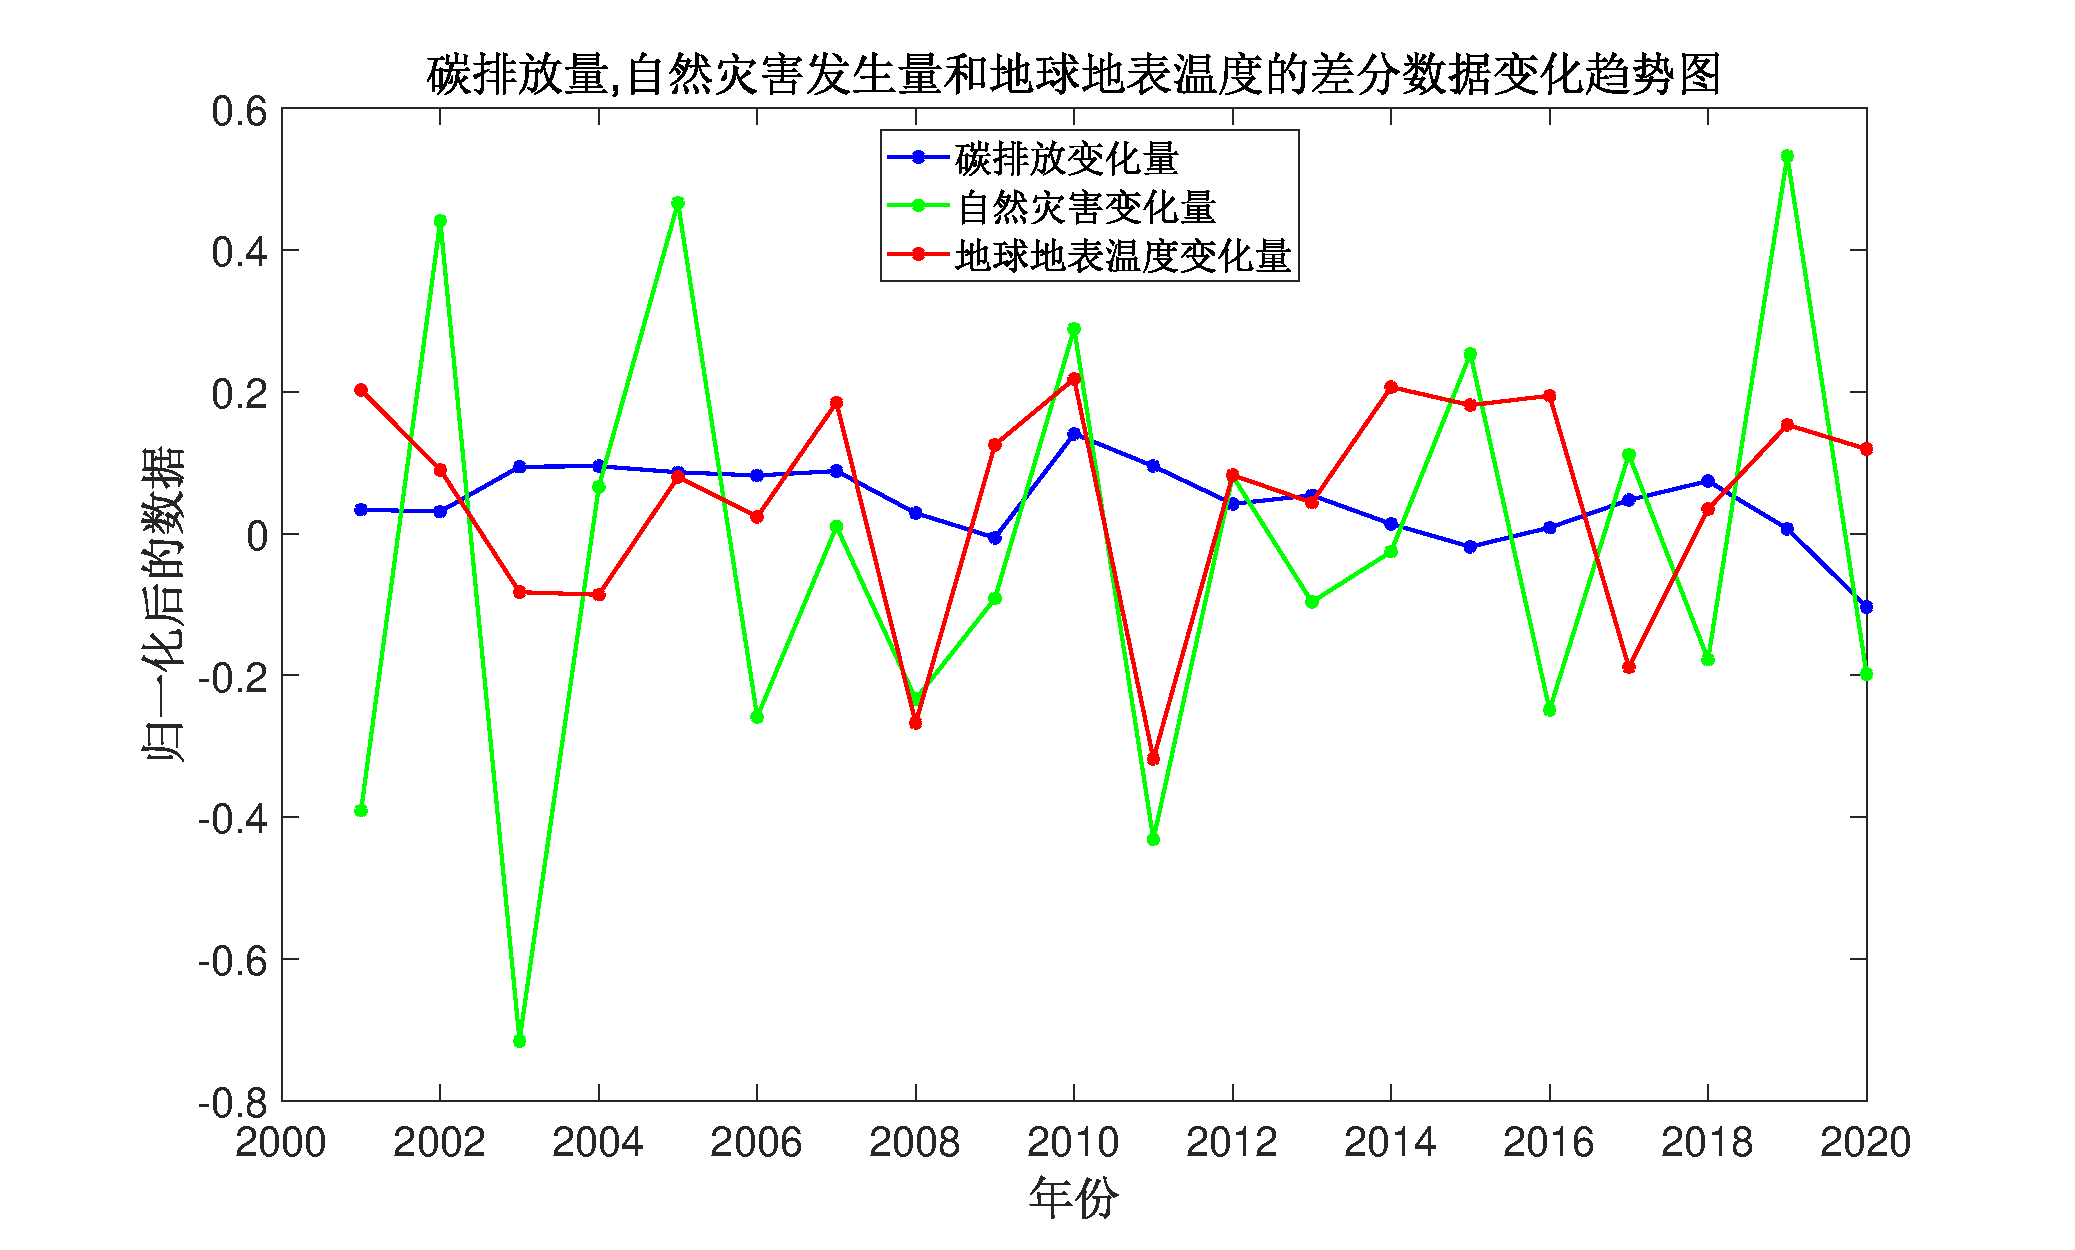
\includegraphics[width=0.50\textwidth]{diff_trend_pro1.eps}}
	\caption{ }
	\label{fig:333i}
\end{figure} 
分析图\ref{fig:图e2}可知从2000年到2020年,全球碳排放量与地球地表温度整体呈上升趋势,初步推断两者为正相关,而全球碳排放量与地球地表温度整体呈下降趋势,因此初步推断自然灾害发生量与全球碳排放量与、球地表温度分别为负相关。因而可以初步推断全球碳排放量、自然灾害发生量与地球地表温度这三个变量,两两之间具有线性关系。

分析图\ref{fig:图e}可知从2000年到2020年,自然灾害发生量的变化量与地球地表温度变化量,两个差分序列具有较高的一致性,即地球地表温度的变化量下降(上升)时,自然灾害发生量的变化量也下降(上升)。初步推断地球地表温度的变化速度与自然灾害发生量的变化速度可能具有一定的关联性。

上述由变量随时间变化的趋势图,可以横向对比,初步推断全球碳排放量、自然灾害发生量与地球地表温度三者间的关系,但结果可能偏离度较大,无法准确表述三者间的关系,因此本文采用Pearson相关性分析,近一步分析三者间的关系。


\subsection{Pearson相关系数模型建立}
\subsubsection{Pearson相关系数}Pearson相关系数可以用来度量两个变量$a$和$b$之间的线性相关关系,其值介于-1到1之间。这里定义两个变量$a$和$b$之间的Pearson相关系数${{C}_{p}}(a,b)$:
\begin{equation}
\label{eq:1}
	{{C}_{p}}(a,b)=\frac{cov(a,b)}{{{\sigma }_{a}}{{\sigma }_{b}}}=\frac{\sum_{i}^{N}{({{a}_{i}}-\bar{a})({{b}_{i}}-\bar{b})}}{\sqrt{\sum_{i}^{N}{{{({{a}_{i}}-\bar{a})}^{2}}}}\sqrt{\sum_{i}^{N}{{{({{b}_{i}}-\bar{b})}^{2}}}}}
\end{equation}
    式\eqref{eq:1}中,N表示变量的样本数目即2000年到2020年的年份数,${{a}_{i}}$和${{b}_{i}}$分别表示$a$和$b$的第$i$个取值,$\bar{a}$和$\bar{b}$分别是$a$和$b$的均值。

	${\mathop{\rm cov}} (a,b)$表示变量$a$和变量$b$间的协方差,用来度量两个变量间变化趋势是否一致,协方差公式如下:
\begin{equation}
\label{eq:4}
	cov(a,b)=\frac{1}{N}\sum_{i}^{N}{({{a}_{i}}-\bar{a})({{b}_{i}}-\bar{b})}
\end{equation}
${{\sigma }_{a}}$和${{\sigma }_{b}}$是a和b的标准差,用来衡量数据集合中数据点的离散程度或波动性的统计量,以变量$a$为例,标准差公式如下:
\begin{equation}
	{{\sigma }_{a}}=\sqrt{\frac{\sum_{i}^{N}{{{({{a}_{i}}-\bar{a})}^{2}}}}{N}}
\end{equation}
\subsubsection{假设检验}
对于Pearson相关性系数${{C}_{p}}(a,b)$,其绝对值越接近于1,证明对应两个变量的相关性越好,以此逻辑,本文构建Pearson相关性分析模型,但对于Pearson相关系数的求解结果,需要通过假设检验来验证Pearson相关性系数是否显著不同于0。本文运用$t$检验进行假设检验,步骤如下:

	\textbf{Step1:} 设置零假设$H_{0}$ 
	
	相关性系数为0,即两个变量之间不存在线性相关关系。
	
	\textbf{Step2:} 设置备择假设$H_{1}$ 
	
	相关性系数不为0,即两个变量之间存在显著的线性相关关系。
	
	\textbf{Step3:} 计算$t$统计量
	
	\begin{equation}
		\label{eq:2}
		t={{C}_{p}}(a,b)\sqrt{\frac{N-2}{1-{{\left [{{{C}_{p}}(a,b)}\right ]}^{2}}}}
	\end{equation}
	式\eqref{eq:2}中,表示相关性系数,$N$表示变量的样本数目。
	\textbf{Step4:}设定置信水平为$95\%$,则显著性水平$\alpha =1-95\%=0.05$
	
	根据样本量$n$和显著性水平$\alpha $ 确定 $t$ 分布的自由度和临界值,依据$t$分布的自由度和临界值选择拒绝域的边界。
	
	\textbf{Step5:}检验$t$ 统计量$t$值是否落在 $t$ 分布的拒绝域内
	
	如果 $t$ 统计量落在拒绝域内,则拒绝零假设,认为两个变量之间存在显著的线性相关关系;否则接受零假设,认为两个变量之间不存在显著的线性相关关系。一般来说,如果 $p$ 值小于显著性水平$\alpha $,就可以拒绝原假设。$p$值是在给定原假设下观察到的统计量或者更极端统计量的概率。
	
	\subsection{Pearson相关系数模型求解}
	\subsubsection{判断全球碳排放量、自然灾害发生量、地球地表温度间的线性相关关系}
	\textbf{Step1:}计算Pearson相关系数
	依照所建立的Pearson相关性分析模型,对全球碳排放量、自然灾害发生量、地球地表温度三个变量进行不重复的两两组合$C_3^2$,由式\eqref{eq:1}分别计算它们的Pearson相关系数为:
	\begin{align*}
		{{C}_{p}}(Carbon,Disaster)=-0.711478242 
	\end{align*}
	\begin{align*}
		{{C}_{p}}(Carbon,Temperature)=0.735122127
	\end{align*}
	\begin{align*}
		{{C}_{p}}(Disaster,Temperature)=-0.355346491
	\end{align*}

将所得Pearson相关系数数据绘制成热力图\ref{fig:corrpro1},图中,颜色越深代表两个变量间的相关性越强,方格中数据为两个变量间的相关系数${{C}_{p}}(a,b)$。
	
	
% TODO: \usepackage{graphicx} required
\begin{figure}[htbp]
	\centering
	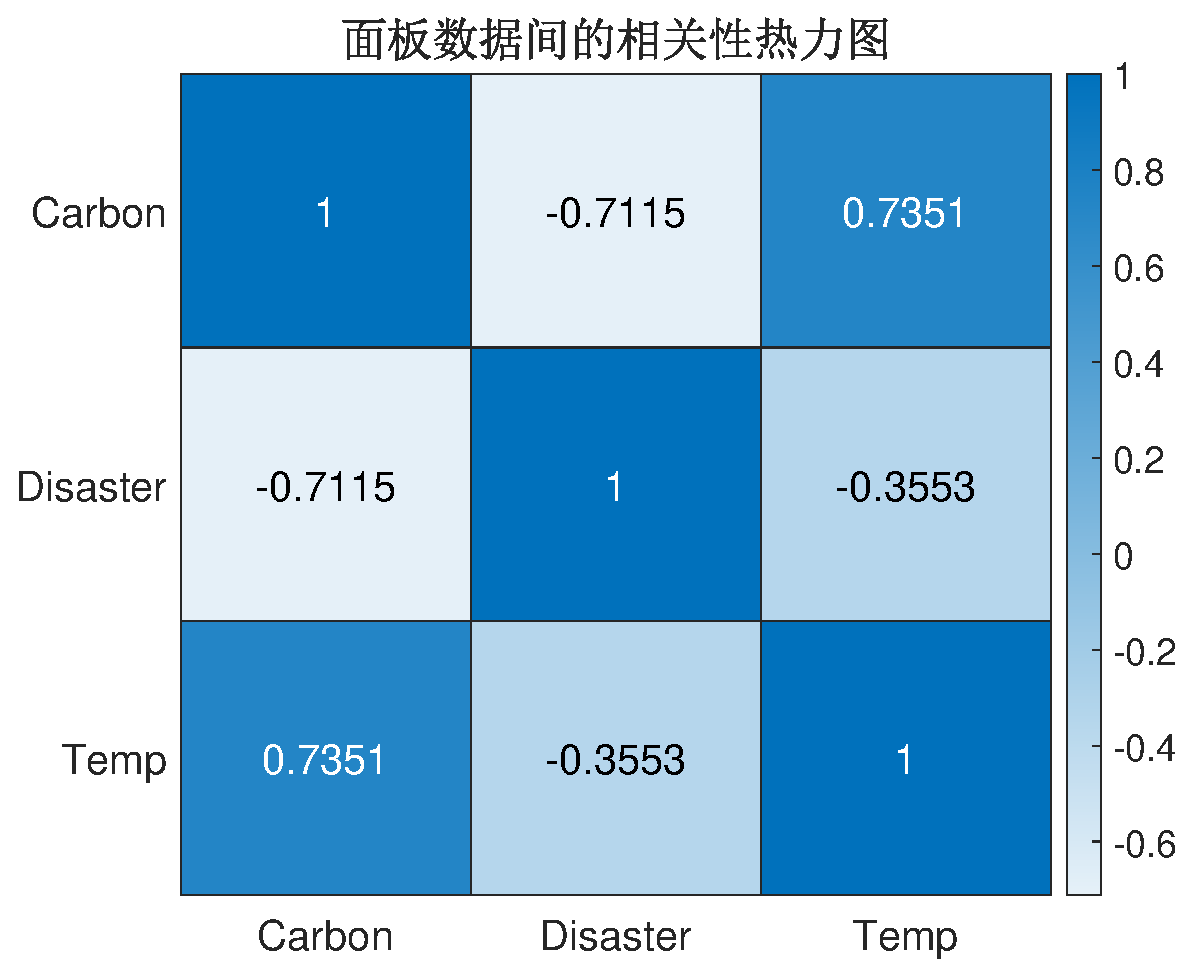
\includegraphics[width=0.6\linewidth]{corr_pro1.eps}
	\caption{全球碳排放量、自然灾害发生量与地球地表温度Pearson相关系数热力图}
	\label{fig:corrpro1}
\end{figure}

	\textbf{Step2:$t$检验}
	
	本文显著性水平$\alpha$取0.05,在此对三者间Pearson相关系数进行$t$检验,由式\eqref{eq:1}计算得出三者间各自的$t$统计量后,查找$t$分布表得到各组的$p$值,并与显著性水平$\alpha $比较,得到表达式如下:
	\begin{align*}
		p(Carbon,Disaster)=0.000298552<\alpha
	\end{align*}
	\begin{align*}
		p(Carbon,Temperature)=0.000146843<\alpha
	\end{align*}
	\begin{align*}
		p(Disaster,Temperature)=0.113926282>\alpha
	\end{align*}
	
	则假设检验结果为:拒绝全球碳排放量与自然灾害发生量不存在显著的线性相关关系这一零假设,拒绝全球碳排放量与地球地表温度不存在显著的线性相关关系这一零假设,接受地球地表温度与自然灾害发生量不存在显著的线性相关关系这一零假设。
	
	\textbf{Step3:}总结
	
	依据图\ref{fig:corrpro1}及假设检验,可知全球碳排放量与地球地表温度具有较强的正相关性,若全球碳排放量上升,地球地表温度也会上升,反之亦然。全球碳排放量与自然灾害发生量具有较强的负相关性,若全球碳排放量降低,自然灾害发生量反而会上升。而自然灾害发生量与地球地表温度不存在显著的线性相关关系。故初步分析所得推断部分正确,更进一步推断为:全球碳排放量与地球地表温度具有正相关性,与自然灾害发生量具有负相关性,自然灾害发生量与地球地表温度不具有相关性。
	
	
	\subsubsection{判断全球碳排放变化量、自然灾害发生变化量、地球地表温度变化量之间的线性相关关系}
	
	\textbf{Step1:}计算Pearson相关系数
	
	具体步骤同\textbf{5.3.1}:依照所建立的Pearson相关性分析模型,对全球碳排放变化量、自然灾害发生变化量、地球地表温度变化量三个变量进行不重复的两两组合$C_3^2$,由式\eqref{eq:1}分别计算它们的Pearson相关系数为:
	
\begin{align*}
	{{C}_{p}}(Carbon,Disaster)=-0.03748184
\end{align*}
\begin{align*}
	{{C}_{p}}(Carbon,Temperature)=-0.27056164
\end{align*}
\begin{align*}
	{{C}_{p}}(Disaster,Temperature)=0.361841976
\end{align*}
	
	其中,$Carbon$表示全球碳排放量,$Disaster$表示自然灾害发生量,$Temperature$表示地球地表温度。将所得Pearson相关系数数据绘制成热力图\ref{fig:corrdiffpro1},图中,颜色越深代表两个变量间的相关性越强,方格中数据为两个变量间的相关系数,数据可视化如下:
	
% TODO: \usepackage{graphicx} required
\begin{figure}[htbp]
	\centering
	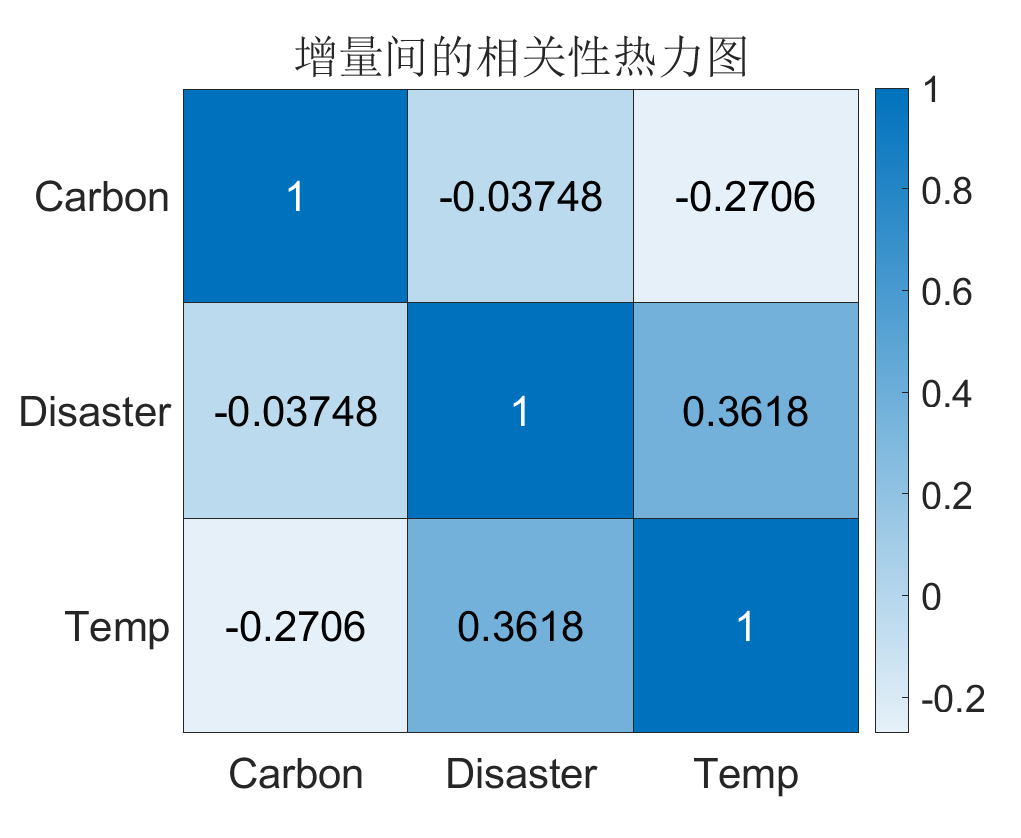
\includegraphics[width=0.7\linewidth]{corr_diff_pro1.eps}
	\caption{全球碳排放变化量、自然灾害发生变化量与地球地表温度变化量Pearson相关系数热力图}
	\label{fig:corrdiffpro1}
\end{figure}





	\textbf{Step2:}$t$检验
	
本文显著性水平$\alpha$取0.05,在此对三者间Pearson相关系数进行$t$检验,由式\eqref{eq:2}计算得出三者间各自的$t$统计量后,查找$t$分布表得到各组的$p$值,并与显著性水平$\alpha $比较,得到表达式如下:
	\begin{align*}
		p(Carbon,Disaster)=0.875335395>\alpha
	\end{align*}
	\begin{align*}
		p(Carbon,Temperature)=0.248599595>\alpha
	\end{align*}
	\begin{align*}
		p(Disaster,Temperature)=0.116956267>\alpha
	\end{align*}
	
	则假设检验结果为:接受全球碳排放变化量与自然灾害发生变化量不存在显著的线性相关关系这一零假设,接受全球碳排放变化量与地球地表温度变化量不存在显著的线性相关关系这一零假设,接受地球地表温度变化量与自然灾害发生变化量不存在显著的线性相关关系这一零假设。
	
	\textbf{Step3:}总结
	
	由假设检验可知全球碳排放变化量、自然灾害发生变化量、地球地表温度变化量两两之间无显著的线性相关关系,初步分析所得推断错误,后续过程不再考虑三者间的关系。
	
	\subsection{插值拟合模型建立与求解}
	\subsubsection{三次样条插值模型建立}
常见的插值方法包括线性插值、拉格朗日插值、牛顿插值、样条插值等,其中三次样条插值,相较于其他常见插值方法,通过三次多项式片段来拟合数据,从而获得连续且具有较高光滑度的插值曲线。故而本文采用三次样条插值建立数学模型,来判断全球碳排放量、自然灾害发生量与地球地表温度三者间的关系。
	    
	三次样条插值是将插值区间内的数据点与相邻区间的数据点之间连接的三次多项式称为样条函数,从而使整个插值区间内的插值曲线是由多个三次多项式片段组成的。本文用表示变量的样本数目,在问题一中即表示2000年到2020年的年份数,设$X_i$为碳排放量数据,$Y_i$为自然灾害发生量数据,$Z_i$为地球地表温度数据。设数据点为$P_i$,问题一中需进行三次样条插值的数据点类型为三维数据点:$(X_i,Y_i,Z_i)$。
	
	三次样条插值拟合模型建立步骤如下:
	
	\textbf{Step1:}
	将N个数据点${P_0},{P_1},{P_2},...,{P_{N - 1}}$的插值区间$[x_0,x_{N-1}]$分成N-1个子区间$[x_0,x_1] ,[x_1,x_2],...,[x_{N-2},x_{N-1}]$,每个子区间内使用一个三次多项式进行插值。
	
	
	
	\textbf{Step2:}
	对于每个子区间$[x_{i-1},x_i]$,其中,$i$表示第$i$个子区间,三次多项式的表达式为:
	\begin{equation}
		\label{eq:5}
		{{S}_{i}}(x)={{a}_{i}}+{{b}_{i}}(x-{{x}_{i}})+{{c}_{i}}(x-{{x}_{i}}{{)}^{2}}+{{d}_{i}}(x-{{x}_{i}}{{)}^{3}},i=0,1,...,N-1.
	\end{equation}
	
	则N个区间对应的三次函数$S(x)$的数学表达式如下:
	
	\begin{equation}
		S(x) = \left\{ \begin{array}{l}
			{s_0}(x) = {a_0} + {b_0}(x - {x_0}) + {c_0}{(x - {x_0})^2} + {d_0}{(x - {x_0})^3},\begin{array}{*{20}{c}}
				{if\begin{array}{*{20}{c}}
						{{x_0} \le x \le {x_1}}
				\end{array}}
			\end{array}\\
			{s_1}(x) = {a_1} + {b_1}(x - {x_1}) + {c_1}{(x - {x_1})^2} + {d_1}{(x - {x_1})^3},\begin{array}{*{20}{c}}
				{}
			\end{array}if\begin{array}{*{20}{c}}
				{{x_1} \le x \le {x_2}}
			\end{array}\\
			{s_2}(x) = {a_2} + {b_2}(x - {x_2}) + {c_2}{(x - {x_2})^2} + {d_2}{(x - {x_2})^3},\begin{array}{*{20}{c}}
				{}
			\end{array}if\begin{array}{*{20}{c}}
				{{x_2} \le x \le {x_3}}
			\end{array}\\
			\vdots \\
			{s_0}(x) = {a_{N - 1}} + {b_{N - 1}}(x - {x_{N - 1}}) + {c_{N - 1}}{(x - {x_{N - 1}})^2} + {d_{N - 1}}{(x - {x_{N - 1}})^3},
			\\if\begin{array}{*{20}{c}}
				{{x_{N - 1}} \le x \le {x_N}}
			\end{array}
		\end{array} \right.
	\end{equation}
	
	\textbf{Step3:}	设置以下条件
	
\begin{equation}
	\label{eq:41}
	\left \{{\begin{matrix}S\left ({{{x}_{i}}}\right )={{y}_{i}},i=0,1,...,N.\\{{S}_{i-1}}\left ({{{x}_{i}}}\right )={{S}_{i}}({{x}_{i}}).\\{{S'}_{i-1}}({{x}_{i}})={{S'}_{i}}({{x}_{i}}).\\{{S''}_{i-1}}({{x}_{i}})={{S''}_{i}}({{x}_{i}}).\\{{S''}_{0}}({{x}_{0}})=0,{{S''}_{N-1}}({{x}_{N}})=0.\\{{S'}_{0}}({{x}_{0}})={{C}_{1}},{{S'}_{N-1}}({{x}_{N}})={{C}_{2}}.\end{matrix}}\right .
\end{equation}
	
	式\eqref{eq:41}作为前提条件,保证了$N$段三次函数必须穿过所有已知节点,且所有节点(除第一节点与最后一个节点)处0、1、2阶连续,同时使三次多项式具有自由边界与固定边界条件。其中$C_i$表示不同的任意常数

	\textbf{Step4:}	得出未知参数方程组
	
	先分别求出函数$S(x)$的一阶导数与二阶导数如下:
\begin{align*}
	\left \{{\begin{matrix}{{S}_{i}}(x)={{a}_{i}}+{{b}_{i}}(x-{{x}_{i}})+{{c}_{i}}(x-{{x}_{i}}{{)}^{2}}+{{d}_{i}}(x-{{x}_{I}}{{)}^{3}}.\\{{{{S}_{i}}}^{'}}(x)={{b}_{i}}+2{{c}_{i}}(x-{{x}_{i}})+3d(x-{{x}_{i}}{{)}^{2}}.\\{{S''}_{i}}(x)=2{{c}_{i}}+6{{d}_{i}}(x-{{x}_{I}}).\end{matrix}}\right .
\end{align*}

	设$h_i=x_{i+1}-x_i, m_i={{S''}_i}(x_i)=2c_i$,由式\eqref{eq:4}推导可得:
	\begin{equation}
		\left\{ {\begin{array}{*{20}{c}}
				{{a_i} = {y_i}}\\
				{{a_i} + {h_i}{b_i} + {h_i}^2{c_i} + {h_i}^3{d_i} = {y_i} + 1}\\
				{{b_i} + 2{h_i}{c_i} + 3h_i^2{d_i} - {b_{i + 1}} = 0}\\
				{2{c_i} + 6{h_i}{d_i} - 2{c_{i + 1}} = 0}\\
				{{c_i} = \frac{{{m_i}}}{2}}\\
				{{d_i} = \frac{{{m_{i + 1}} - {m_i}}}{{6{h_i}}}}\\
				{{b_i} = \frac{{{y_{i + 1}} - {y_i}}}{{{h_i}}} - \frac{{{h_i}}}{2}{m_i} - \frac{{{h_i}}}{6}({m_{i + 1}} - {m_i})}\\
				{{h_i}{m_i} + 2({h_i} + {h_{i + 1}}){m_{i + 1}} + {h_{i + 1}}{m_{i + 2}} = 6[\frac{{{y_{i + 2}} - {y_{i + 1}}}}{{{h_{i + 1}}}} - \frac{{{y_{i + 1}} - {y_i}}}{{{h_i}}}]}
		\end{array}} \right.
	\end{equation}
	\textbf{Step5:}对数据降维
	
	由于问题一中数据点$(X_i,Y_i,Z_i)$为三维数据,故在此对其降维,将三维坐标在空间中的点$(X_i,Y_i,Z_i)$ 连接起来形成一维向量$[X_i,Y_i,Z_I)$,从而方便处理。同时,在插值拟合结束后,需要依照拟合曲面的平滑性对插值曲面的插值效果进行评估。
	
	\subsubsection{三次样条插值模型求解}
	对于$(X_N,Y_N,Z_N)$这一三维数据类型,本文通过上述所建立的三次样条插值模型,首先对三维数据进行降维处理,后代入三次多项式\eqref{eq:5}:
	\begin{align*}
		{{S}_{i}}(x)={{a}_{i}}+{{b}_{i}}(x-{{x}_{i}})+{{c}_{i}}(x-{{x}_{i}}{{)}^{2}}+{{d}_{i}}(x-{{x}_{i}}{{)}^{3}},i=0,1,...,N-1.
	\end{align*}
	通过条件方程组\eqref{eq:4}
	\begin{align*}
		\left \{{\begin{matrix}S\left ({{{x}_{i}}}\right )={{y}_{i}},i=0,1,...,N.\\{{S}_{i-1}}\left ({{{x}_{i}}}\right )={{S}_{i}}({{x}_{i}}).\\{{S'}_{i-1}}({{x}_{i}})={{S'}_{i}}({{x}_{i}}).\\{{S''}_{i-1}}({{x}_{i}})={{S''}_{i}}({{x}_{i}}).\\{{S''}_{0}}({{x}_{0}})=0,{{S''}_{N-1}}({{x}_{N}})=0.\\{{S'}_{0}}({{x}_{0}})={{C}_{1}},{{S'}_{N-1}}({{x}_{N}})={{C}_{2}}.\end{matrix}}\right .
	\end{align*}


	绘制插值拟合曲面坐标图的不同方向视图如图\ref{fig:chazhi}所示:
	
\begin{figure}[htbp]
	\centering
	\subcaptionbox{插值拟合3D图\label{fig:图a}}
	{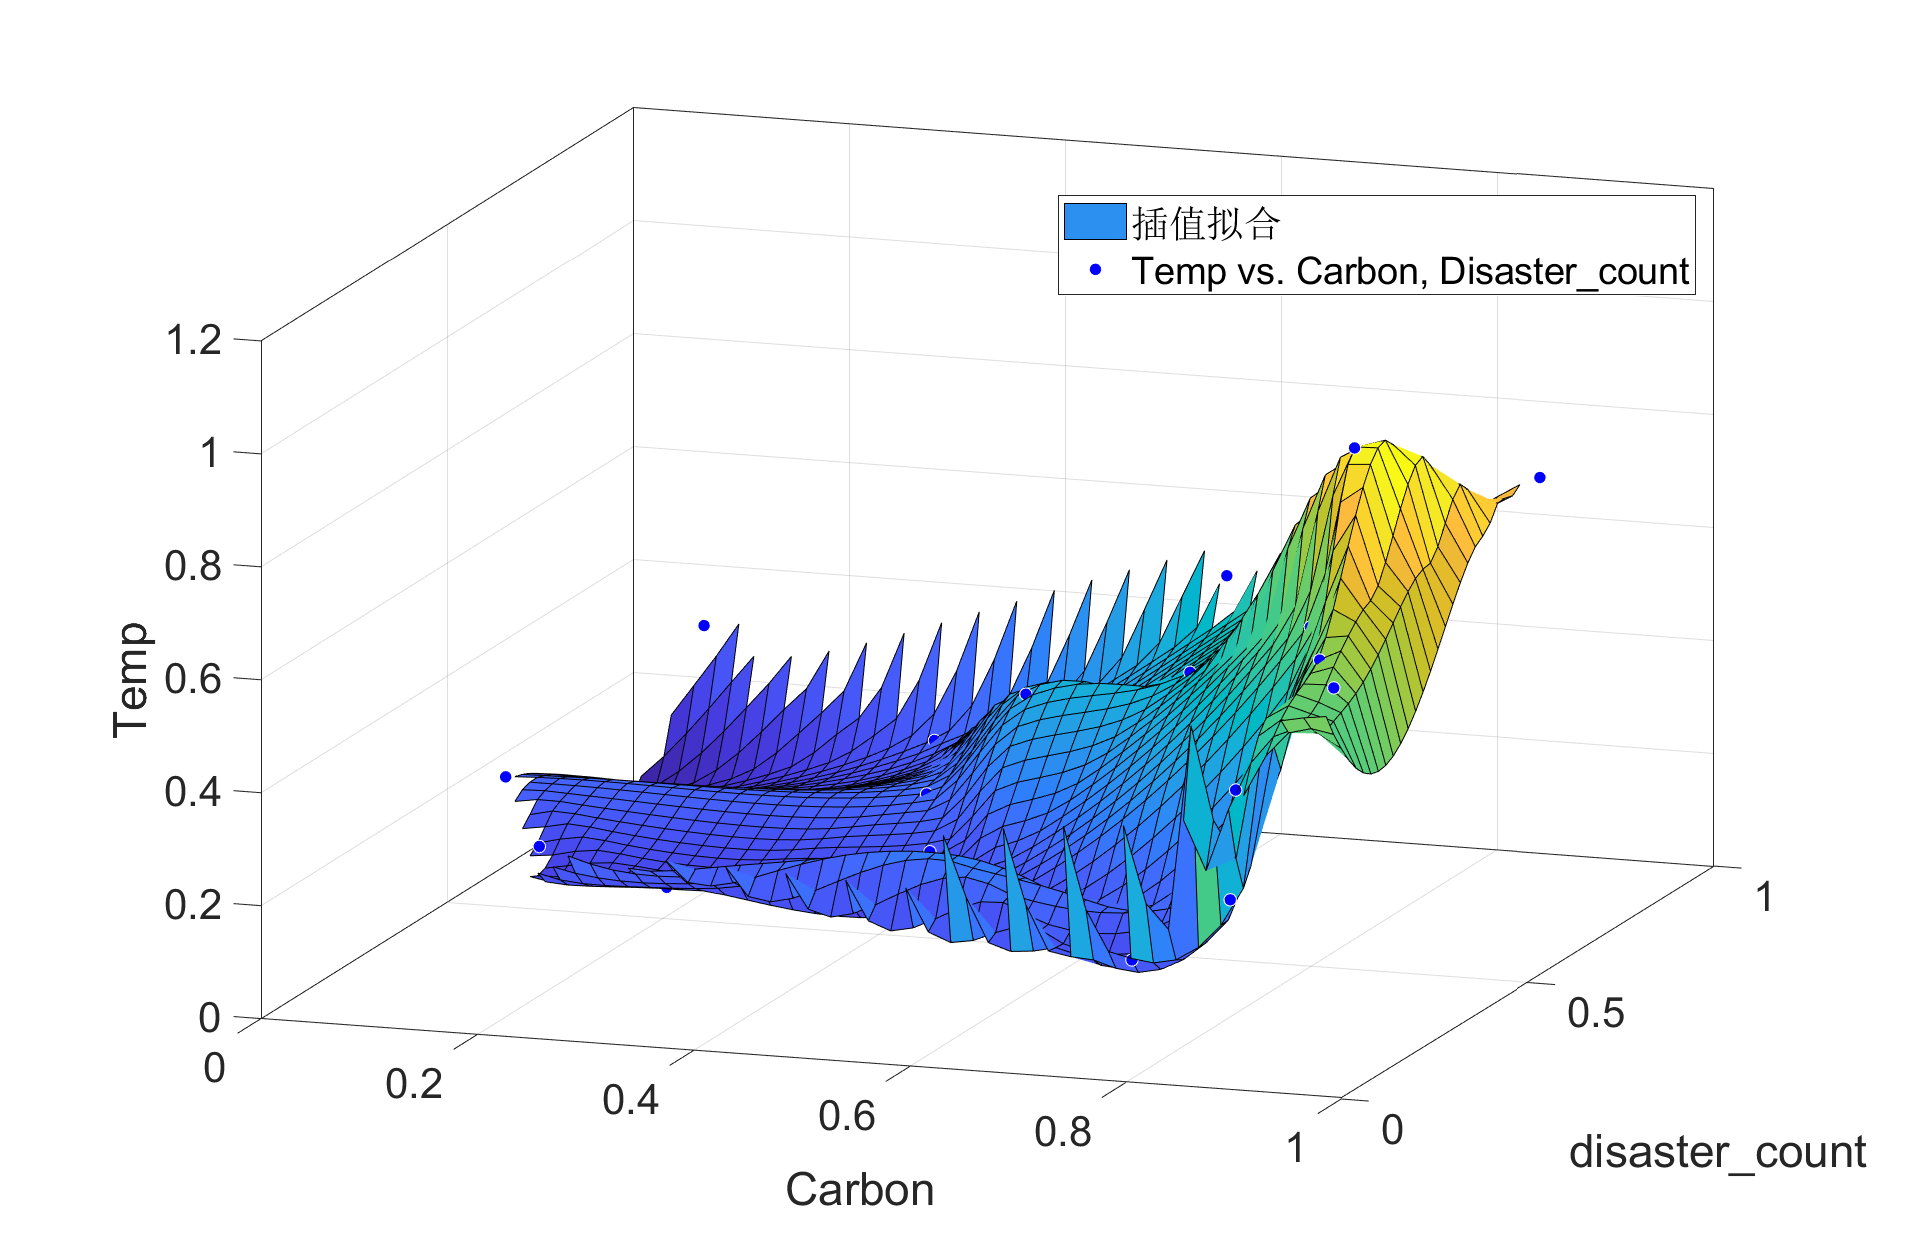
\includegraphics[width=.4\textwidth]{Interpolation.eps}}
	\subcaptionbox{碳排放量与地球地表温度\label{fig:图b}}
	{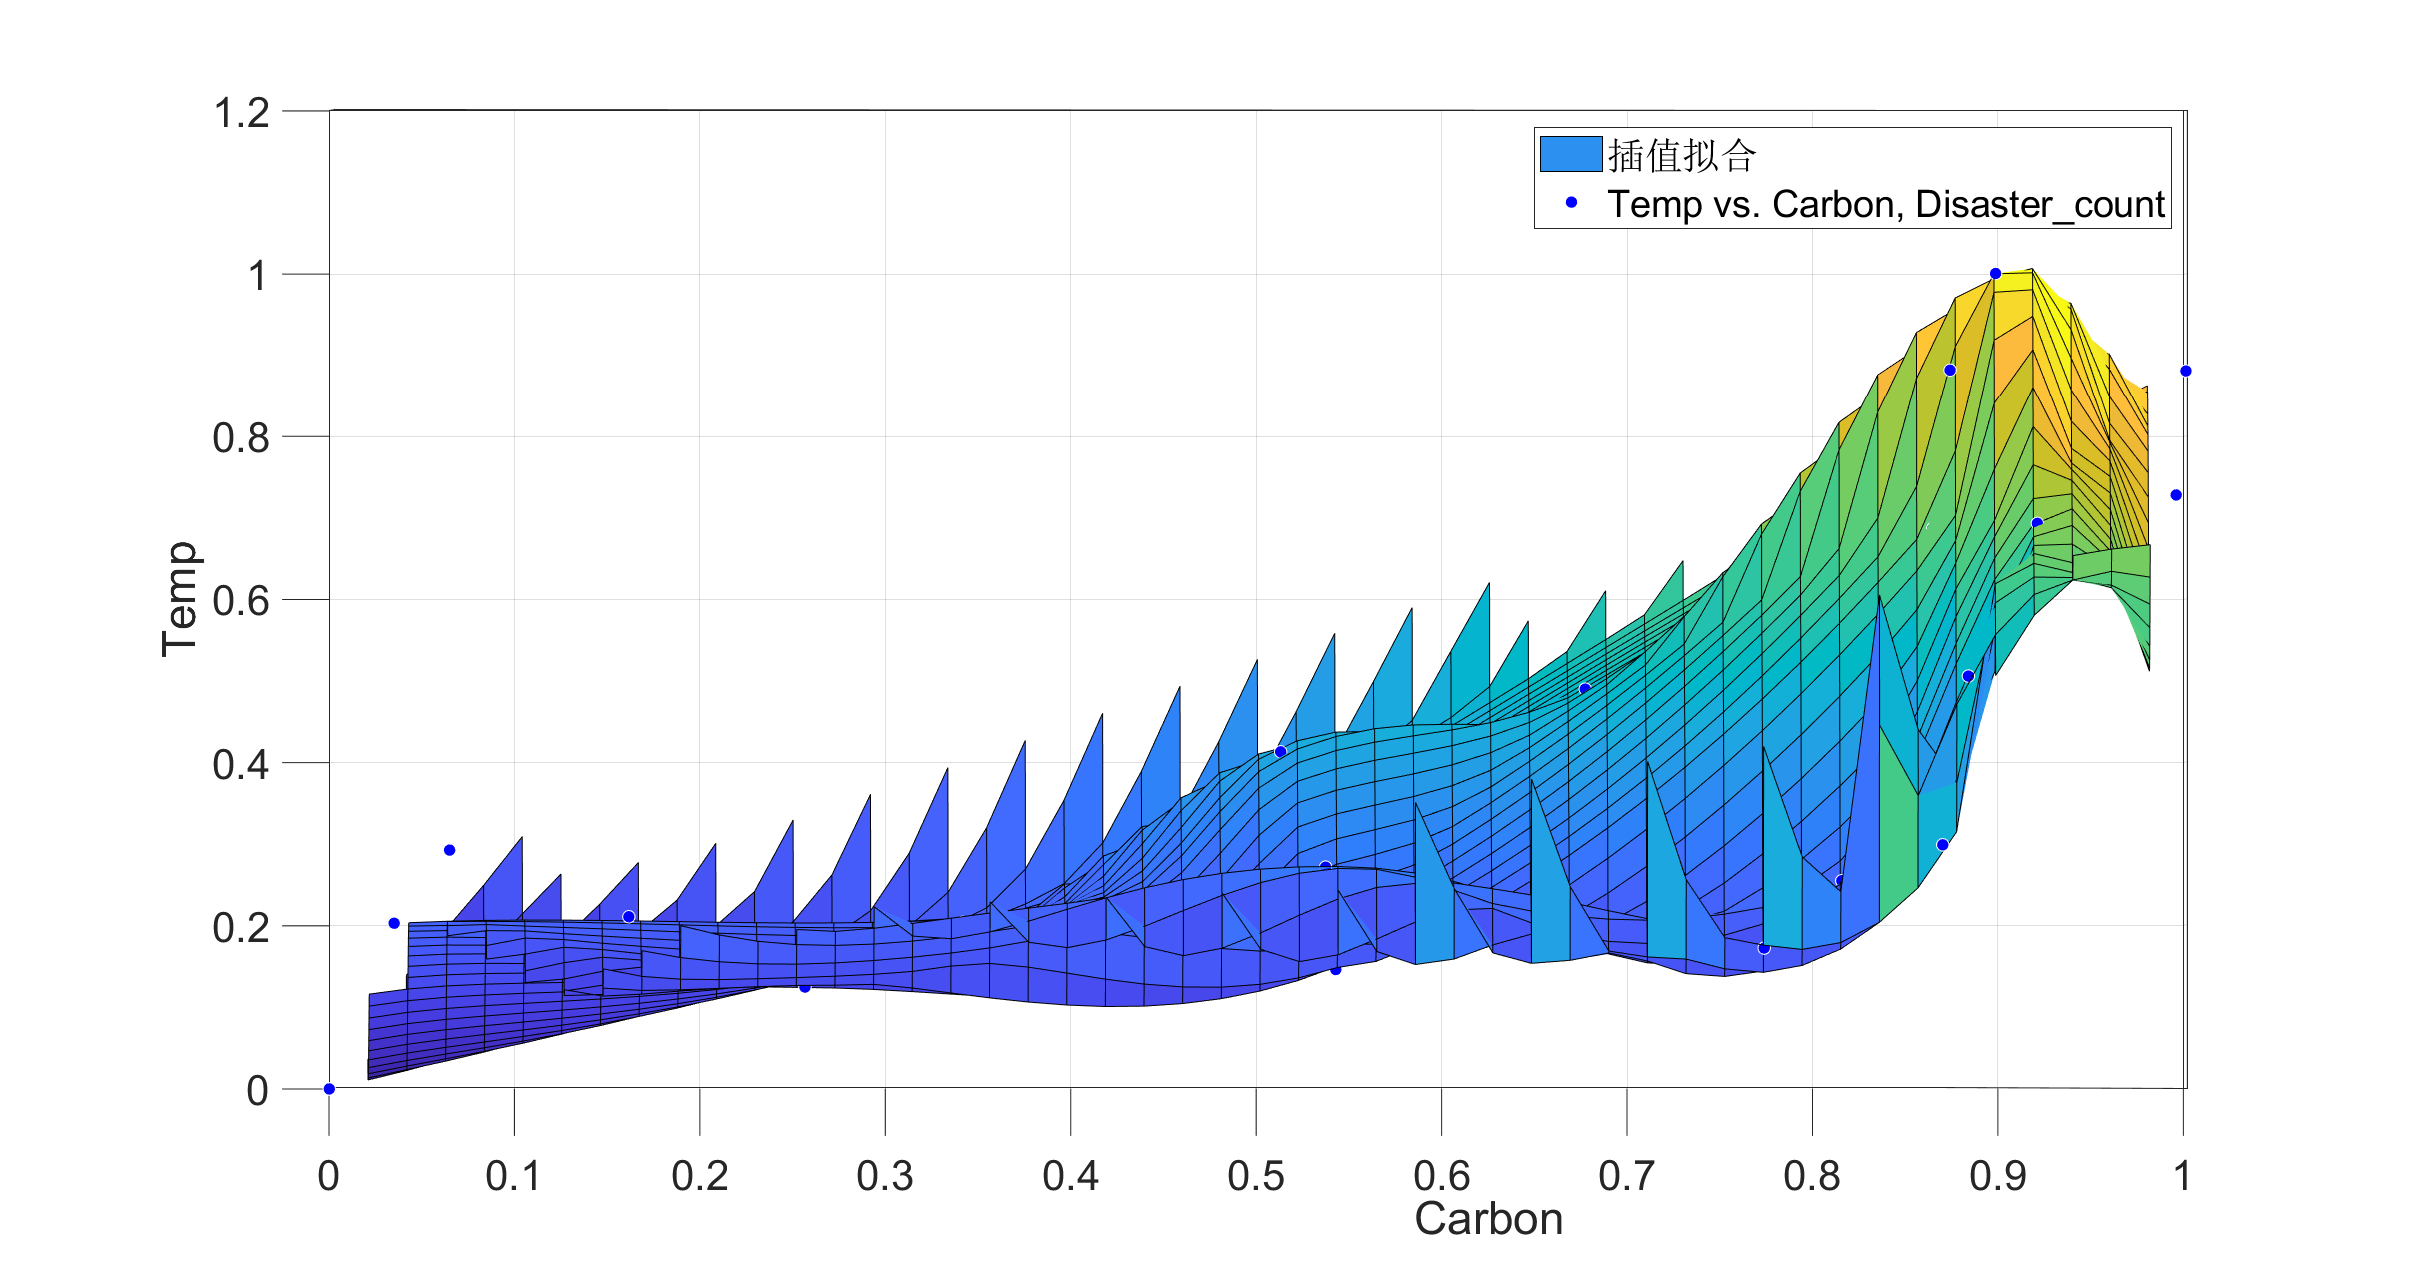
\includegraphics[width=.4\textwidth]{carbon_Temp.eps}}
	\subcaptionbox{碳排放量与自然灾害发生量\label{fig:图c}}
	{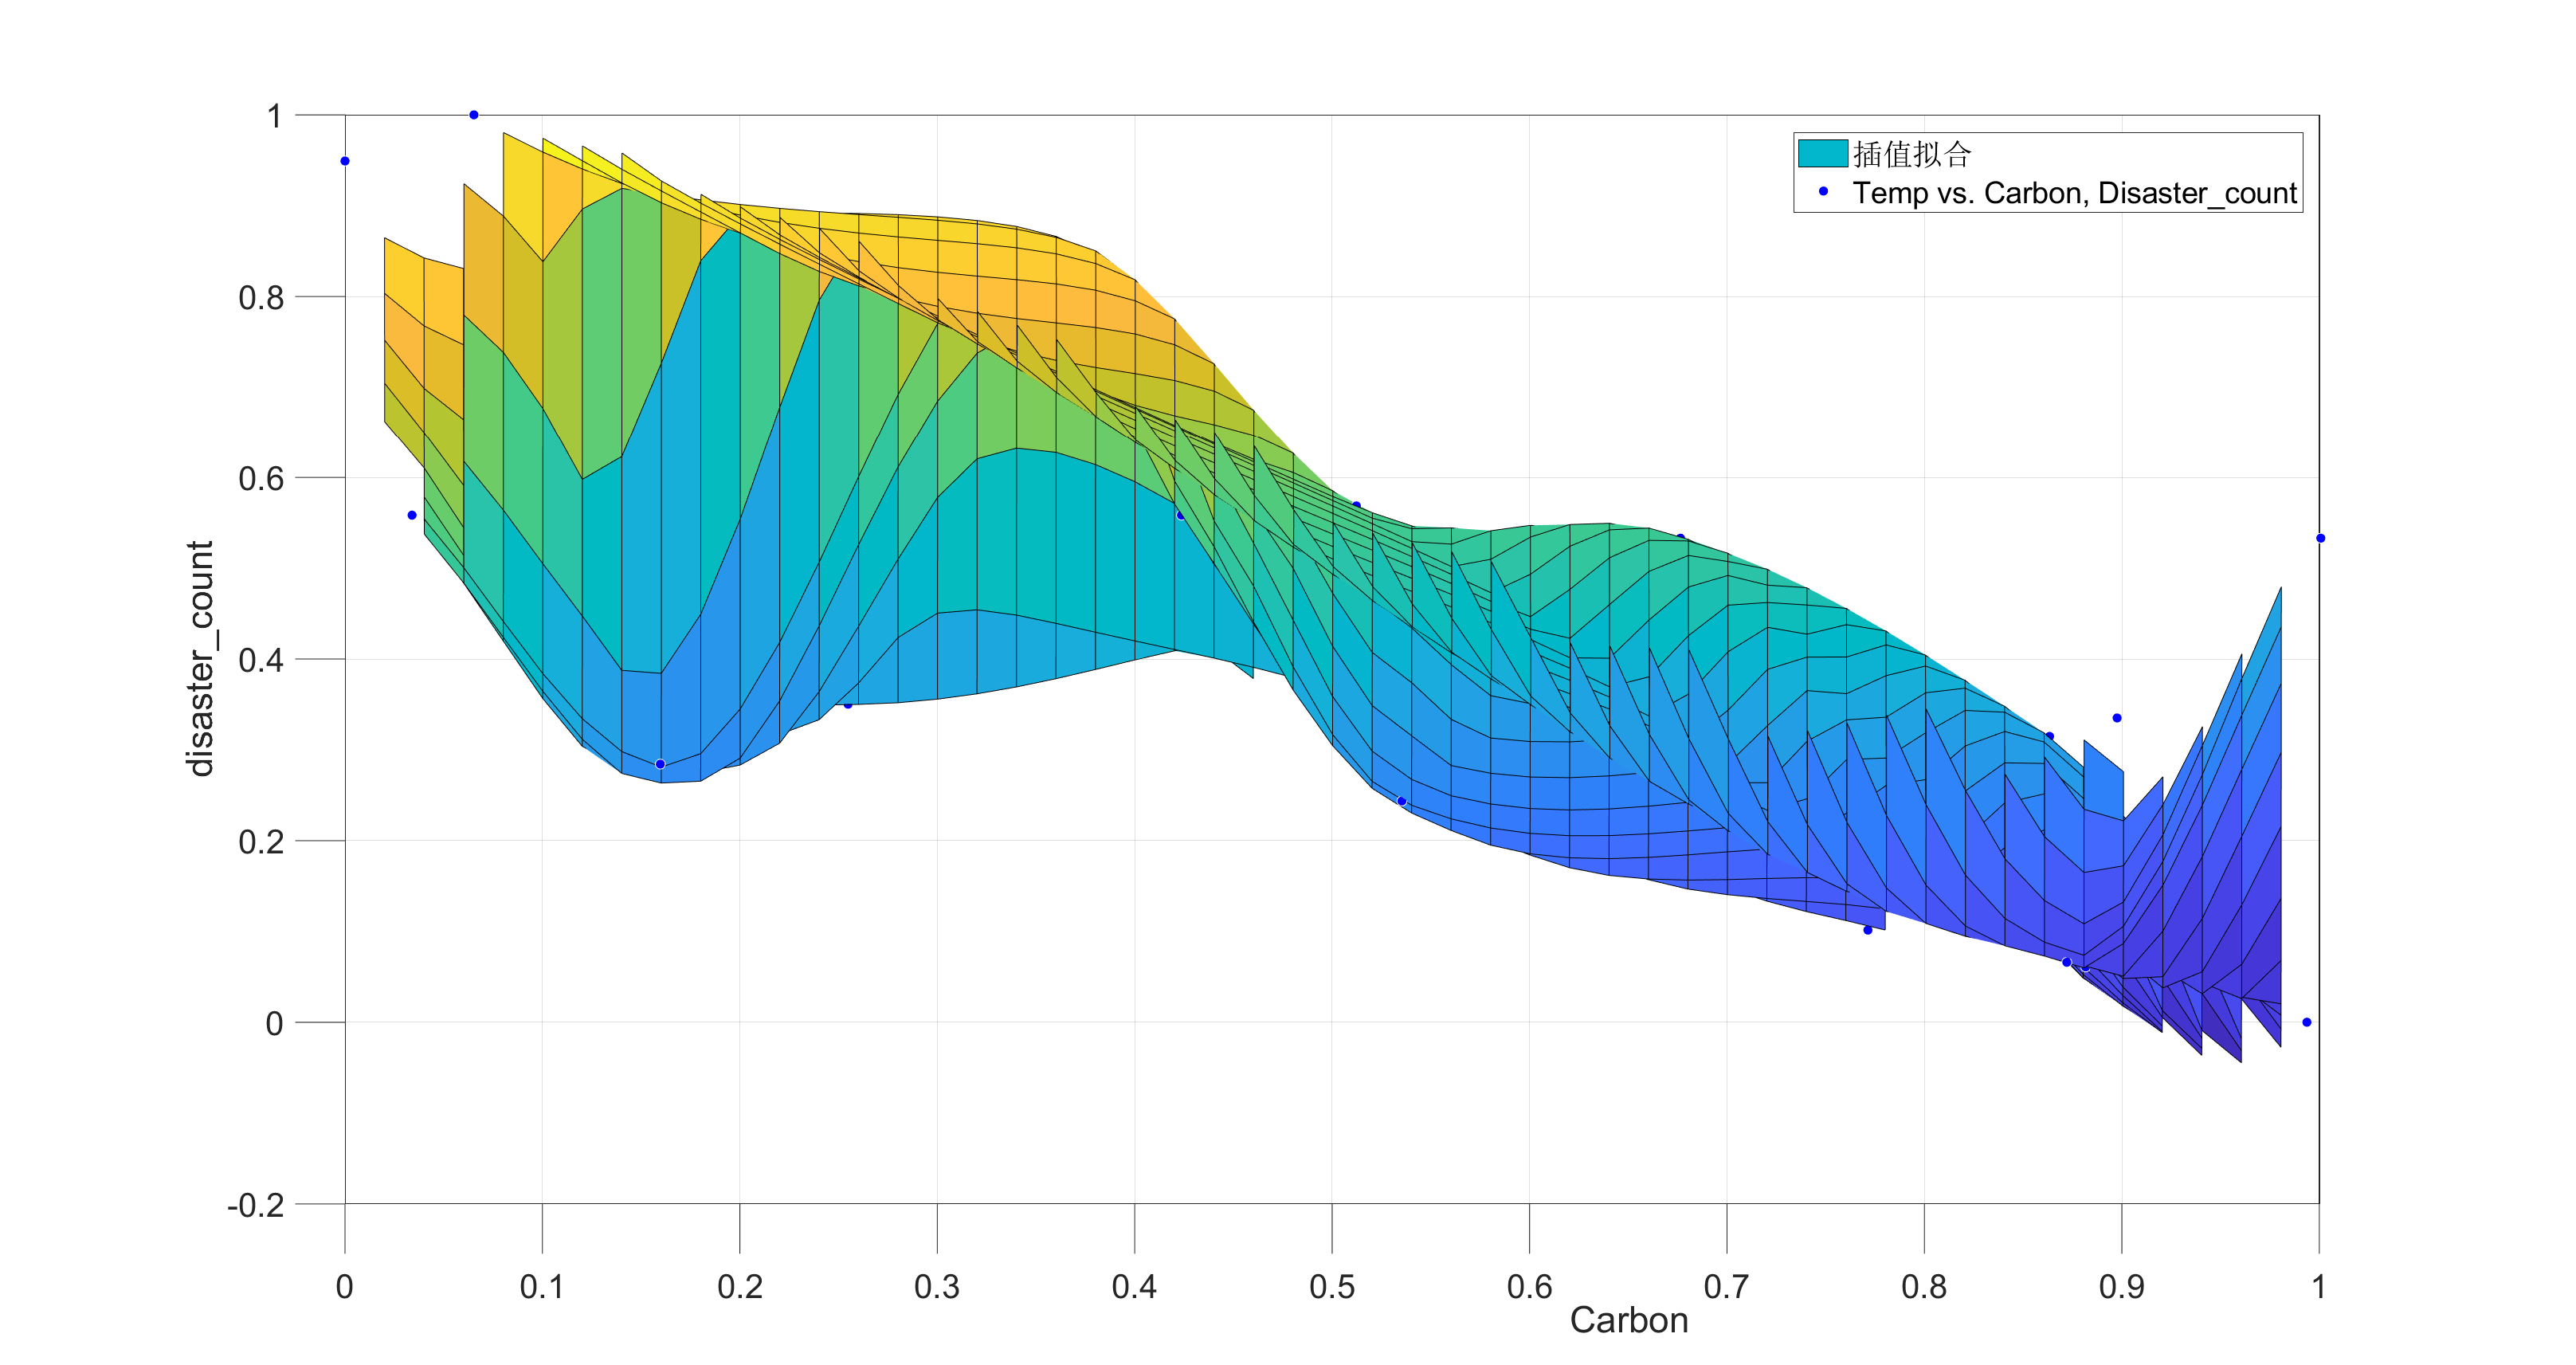
\includegraphics[width=.4\textwidth]{carbon_disaster.eps}}
	\subcaptionbox{自然灾害发生量与地球地表温度变化\label{fig:图d}}
	{\includegraphics[width=.4\textwidth]{disaster_Temp.jpg}}
	\caption{不同方向视图}\label{fig:不同方向视图}
	\label{fig:chazhi}
\end{figure} 

    由图不难看出,随着碳排放量的升高,地球地表温度变化具有升高的趋势,自然灾害的发生量具有下降的趋势。对于自然灾害发生量和地球地表温度变化,并不能由图示看出明显的线性相关性,故插值拟合的结果与Pearson相关系数模型所得结果相互佐证,最终得出全球碳排放量、自然灾害发生量与地球地表温度之间的关系为:全球碳排放量与自然灾害发生量、地球地表温度变化均具有较强的线性相关性,其中全球碳排放量与地球地表温度变化呈正相关,与自然灾害发生量呈负相关。对于地球地表温度变化与自然灾害发生量,两者间并不能得到明显且单一的线性关系。
    
\subsection{最小二乘回归模型建立与求解}
一元最小二乘回归的一般形式为:
\begin{align*}
	f(x) = ax +b
\end{align*}

自然灾害发生量与碳排放量的关系:
	\begin{align*}
		 y = -0.61039 x + 0.744554
	\end{align*}

地球地表温度与碳排放量的关系:
	\begin{align*}
 		y = 0.63013 x + 0.040607
	\end{align*}

两者的最小二乘回归拟合图如图\ref{fig:ols952}所示:

\begin{figure}[h]
	\centering
	\includegraphics[width=0.8\linewidth]{../code/pics/pro1/ols_95_2}
	\caption{最小二乘回归拟合图}
	\label{fig:ols952}
\end{figure}


两者的解释方差都在95\%以内,可见存在线性关系。

%%%%%%%%%%%%%%%%%%%%%%%%%%%%%%%%%%%%%%%%%%%%%%%%%%%%%%%%%%%%% 

\section{问题二的模型的建立和求解}

% TODO: \usepackage{graphicx} required
\begin{figure}[htbp]
	\centering
	\includegraphics[width=0.7\linewidth]{framework2}
	\caption{问题二求解流程图}
	\label{fig:framework2}
\end{figure}


\subsection{数据预处理}
    对于全球碳排放量、全球甲烷排放量,全球一氧化氮排放量和全球温室气体排放量四个附录文件,由于其中数据准确性、完整性和一致性都较差,故需要进行数据预处理,以数据清洗、集成、归约、变换等方式提高数据质量。本文通过对全球碳排放量、全球甲烷排放量,全球一氧化氮排放量和全球温室气体排放量数据进行清洗,去除其中的无效数据,对于有效数据的部分缺失值采用均值插补法进行补全。然后通过数据属性选择的方法,删除与全全球碳排放量、全球甲烷排放量,全球一氧化氮排放量和全球温室气体排放量等有效数据不相关或冗余的属性从而进行数据归约。最后通过数据标准化,将全球碳排放量、全球甲烷排放量,全球一氧化氮排放量和全球温室气体排放量等数据按比例缩放,对数据进行无量纲处理,完成数据变换,运用$0-1$标准化方法对原始数据进行线性变换,使结果落在$[0,1]$区间内,原始数据转换的函数如下:
    \begin{align*}
    	{{k}^{*}}=\frac{k-\min{k}}{\max{k}-\min{k}}
    \end{align*}
\subsection{比较全球碳排放量、全球甲烷排放量,全球一氧化氮排放量和全球温室气体排放量}
	    由于问题二要比较一氧化氮排放量、甲烷排放量、碳排放量,故本文在进行数据归一化时过程中保留了1990年到2020年间三者的原始有效数据,并绘制出全球碳排放量、全球甲烷排放量,全球一氧化氮排放量和全球温室气体排放量原始数据随年份变化对比图\ref{fig:图a1}。对于预处理后的数据,本文选择截取其1990年到2020年间30年的数据进行数据可视化,绘制出全球碳排放量、全球甲烷排放量,全球一氧化氮排放量和全球温室气体排放量数据归一化后随年份变化对比图\ref{fig:图b1},趋势图如下:
\begin{figure}[htbp]
	\centering
	\subcaptionbox{\label{fig:图a1}}
	{\includegraphics[width=.4\textwidth]{minmax3_trend_pro2.eps}}
	\subcaptionbox{\label{fig:图b1}}
	{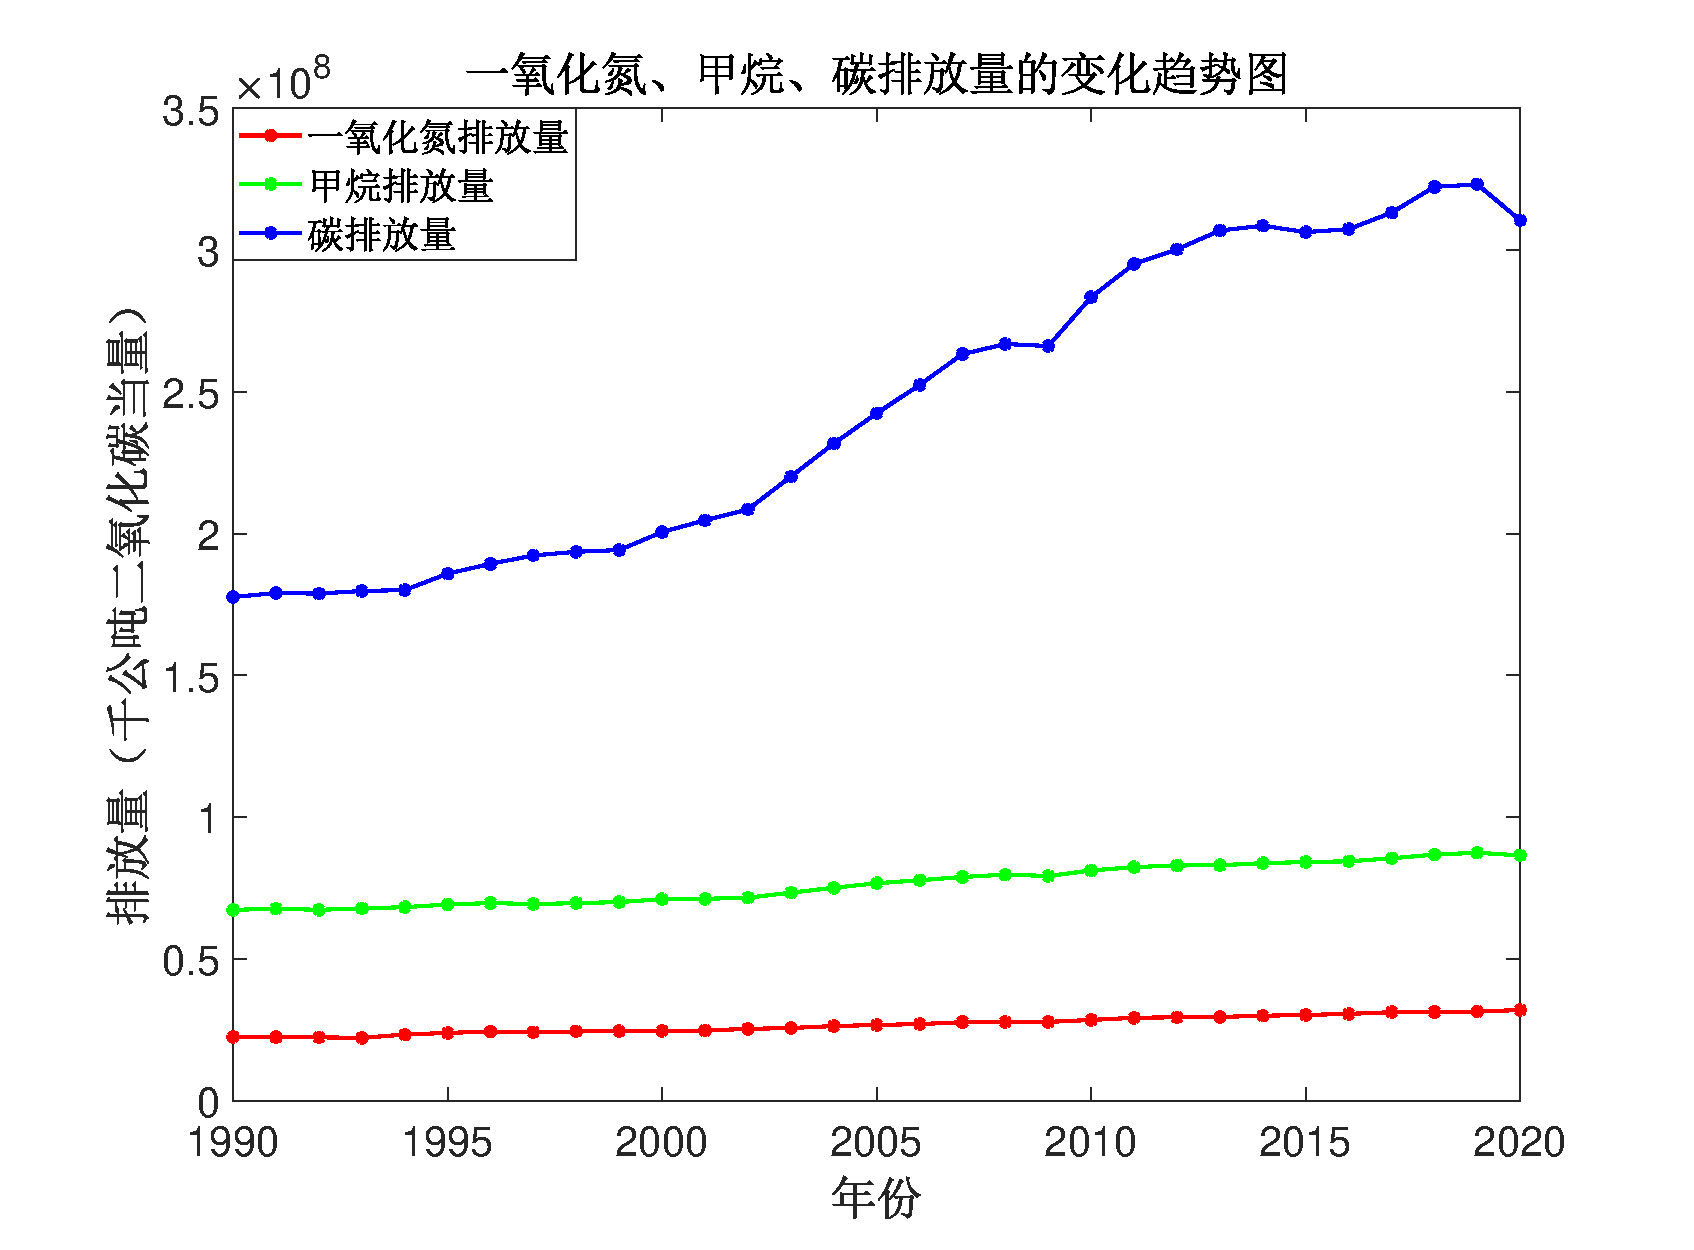
\includegraphics[width=.4\textwidth]{raw3_trend_pro2.eps}}
\label{fig:双图2}
\end{figure} 

    分析图\ref{fig:图a1}易得,随着时间推移,全球碳排放量的原始数据远远大于甲烷与一氧化氮的排放量,且三者的排放量都逐年增加。分析图\ref{fig:图b1}可得,在数据归一化后,一氧化氮、甲烷、碳排放量三者各自每一年相较于前一年的增幅大致相同,变相说明了全球温室气体排放量可能是逐年递增的。
    
  \subsection{建立评价模型}
	\subsubsection{数据可视化}
对于全球碳排放量、全球甲烷排放量,全球一氧化氮排放量和全球温室气体排放量,本文截取四个变量从2010年到2020年10年间的有效数据,如表\ref{tab:1}所示:
	\begin{table}[htbp]
	\centering
	\caption{2010-2020年的一氧化氮排放量、甲烷排放量、碳排放量与全球温室气体排放量}
	\begin{tabular}{cccc} 
		\hline
		NO          & CH4         & C           & Global       \\ 
		\hline
		28483412.62 & 81197101.5  & 283467660.8 & 920453.5038  \\
		29250651.27 & 82400248.01 & 295140816.4 & 944926.7947  \\
		29426316.02 & 82965892.06 & 300299863.1 & 957645.4161  \\
		29538122.92 & 83058240.37 & 306940989   & 969870.6091  \\
		29968173.64 & 83777380.62 & 308628456.2 & 978397.9685  \\
		30243935.02 & 84193604.08 & 306365564.6 & 973994.7895  \\
		30620325.23 & 84435561.23 & 307416548.5 & 974113.2761  \\
		31218087.49 & 85506705.18 & 313231764.6 & 989535.9583  \\
		31224261.39 & 86797389.2  & 322343484.9 & 1009034.217  \\
		31461311.28 & 87461366.76 & 323190967   & 1010968.234  \\
		31986264.1  & 86516874.62 & 310528346   & 975822.7197  \\
		\hline
	\end{tabular}
	\label{tab:1}
\end{table}


绘制成如图\ref{fig:trendpro2}所示的变化趋势图:

% TODO: \usepackage{graphicx} required
\begin{figure}[htbp]
	\centering
	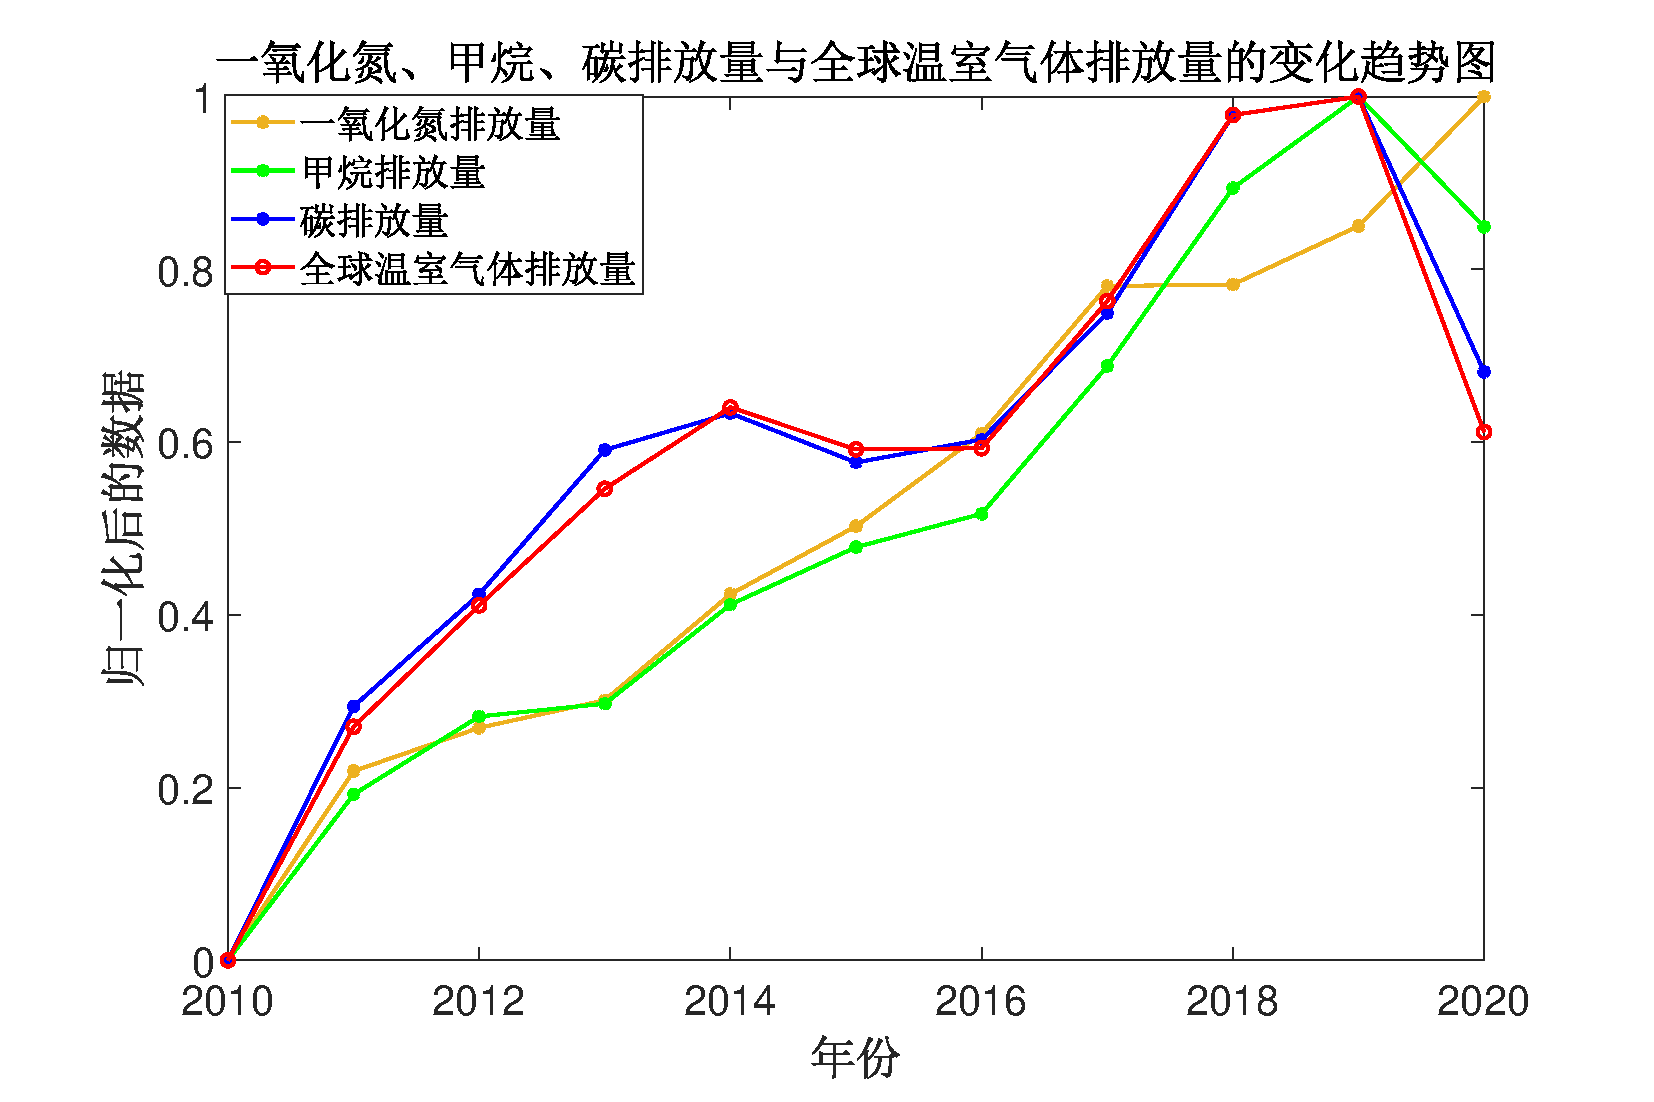
\includegraphics[width=0.7\linewidth]{trend_pro2.eps}
	\caption{一氧化氮排放量、甲烷排放量、碳排放量与全球温室气体排放量变化趋势图}
	\label{fig:trendpro2}
\end{figure}

分析图\ref{fig:trendpro2}发现,碳排放量与全球温室气体排放量的折线具有高度相似性,相较之下,甲烷排放量、一氧化氮排放量与全球温室气体排放量的折线重合点较少,故初步推断,在图示四个变量中,与全球温室气体排放量相关性最高的点可能是全球碳排放量。现通过Pearson相关系数建立评价模型来佐证初步推断。
\subsubsection{建立Pearson相关系数评价模型}
	    基于问题一所建立的Pearson相关系数模型,本文选择用变量的相关性来构建评价模型。通过过式\eqref{eq:6}计算全球碳排放量、全球甲烷排放量,全球一氧化氮排放量和全球温室气体排放量的Pearson相关系数,计算公式如下:
	   \begin{equation}
	   	\label{eq:6}
	   	{{C}_{p}}(a,b)=\frac{cov(a,b)}{{{\sigma }_{a}}{{\sigma }_{b}}}=\frac{\sum_{i}^{N}{({{a}_{i}}-\bar{a})({{b}_{i}}-\bar{b})}}{\sqrt{\sum_{i}^{N}{{{({{a}_{i}}-\bar{a})}^{2}}}}\sqrt{\sum_{i}^{N}{{{({{b}_{i}}-\bar{b})}^{2}}}}}
	   \end{equation}
	   
	   
	   	依照所建立的Pearson相关性分析模型,对全球碳排放量、全球甲烷排放量,全球一氧化氮排放量和全球温室气体排放量四个变量进行不重复的两两组合$C_3^2$,由式\eqref{eq:6}分别计算它们的Pearson相关系数为:
	   
	   \begin{table}[htbp]
	   	\centering
	   	\caption{一氧化氮、甲烷、碳排放量与全球温室气体排放量的 Pearson 相关性矩阵}
	   	\begin{tabular}{c|cccc} 
	   		\hline
	   		& NO       & CH4      & C                 & Global    \\ 
	   		\hline
	   		NO     & 1        & 0.962071 & 0.851835          & 0.830449  \\
	   		CH4    & 0.962071 & 1        & 0.925256          & 0.913004  \\
	   		C      & 0.851835 & 0.925256 & 1                 & 0.995995  \\
	   		Global & 0.830449 & 0.913004 & \textbf{0.995995} & 1         \\
	   		\hline
	   	\end{tabular}
	   \end{table}
	   
	   
	   其中,C表示全球碳排放量,CH4表示全球甲烷排放量,NO表示全球一氧化氮排放量,Global表示全球温室气体排放量。
	   
	   将所得Pearson相关系数数据绘制成热力图\ref{fig:corrpro2},图中颜色越深代表两个变量间的相关性越强,方格中数据为两个变量间的相关系数。
	   % TODO: \usepackage{graphicx} required
	   
	   \begin{figure}[htbp]
	   	\centering
	   	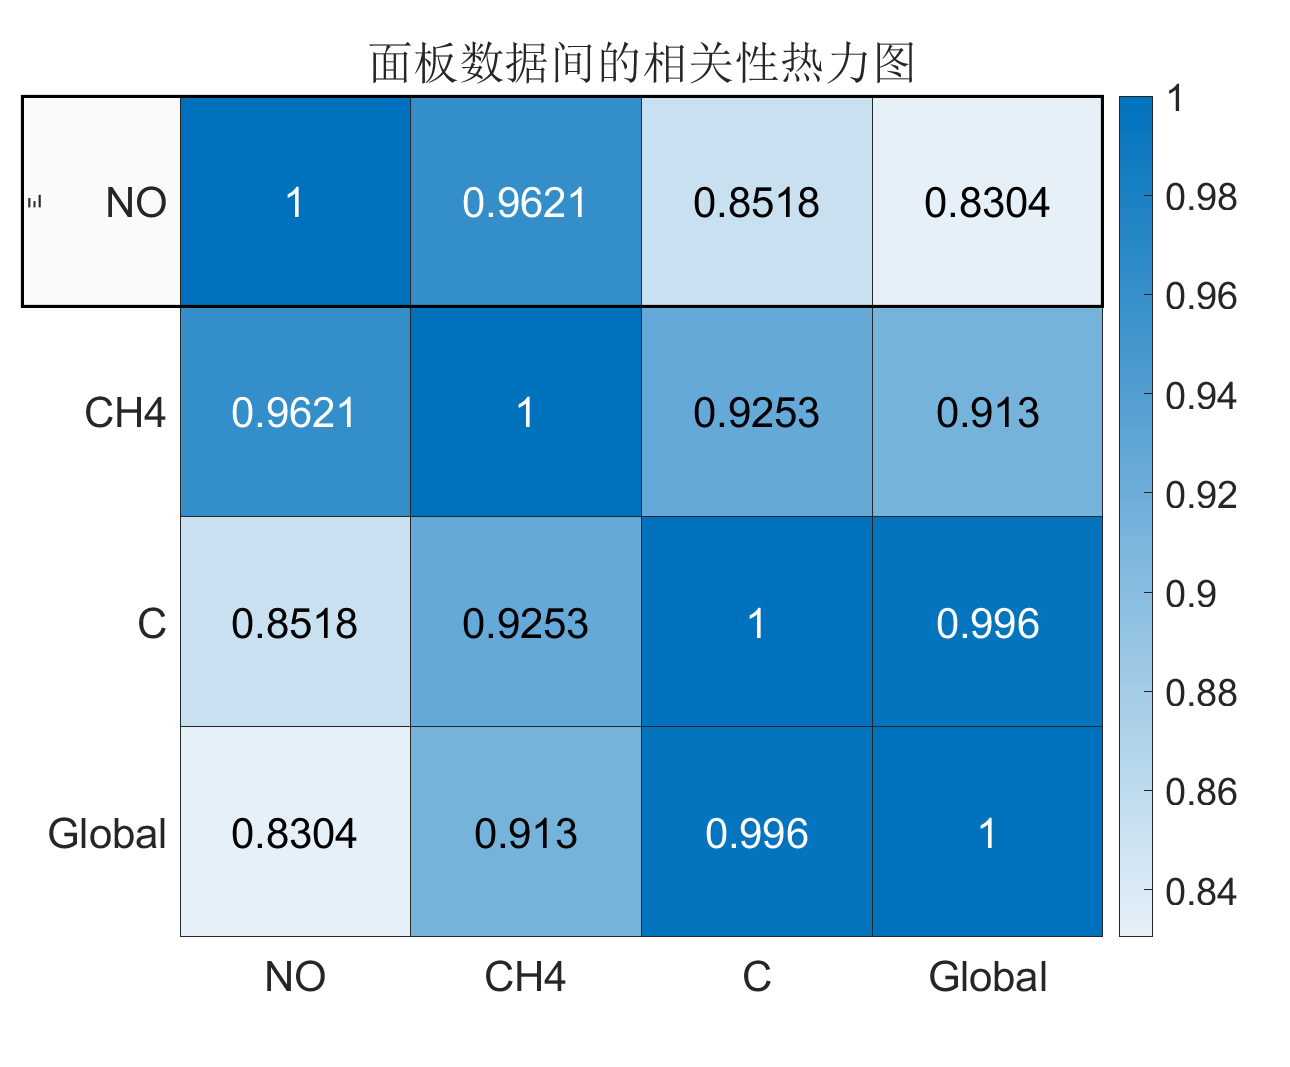
\includegraphics[width=0.6\linewidth]{corr_pro2.eps}
	   	\caption{面板数据间的相关性热力图}
	   	\label{fig:corrpro2}
	   \end{figure}
	   
对图\ref{fig:corrpro2}简单分析,可以发现,对于全球温室气体排放量,和全球碳排放量、全球甲烷排放量,全球一氧化氮排放量中相关系数最高的为碳排放量,后需进行假设检验证明所得结果的可信度。
	   
	   
	   
\subsubsection{$t$检验}
	对计算所得的相关系数进行假设检验,计算各组相关系数的$t$ 统计量:
	\begin{equation}
		\label{eq:7}
		t={{C}_{p}}(a,b)\sqrt{\frac{N-2}{1-{{\left [{{{C}_{p}}(a,b)}\right ]}^{2}}}}
	\end{equation}
	检验$t$ 统计量$t$值是否落在 $t$ 分布的拒绝域内。即检验 $p$ 值是否小于显著性水平$\alpha $,如果 $t$ 统计量落在拒绝域内,则拒绝零假设,认为两个变量之间存在显著的线性相关关系;否则接受零假设,认为两个变量之间不存在显著的线性相关关系。
	
	
本文对于所得全球温室气体排放量与全球碳排放量、全球甲烷排放量,全球一氧化氮排放量各自的相关系数进行$t$检验。分别设置零假设为:全球碳排放量与全球温室气体排放量不存在显著的线性相关关系,全球甲烷排放量与全球温室气体排放量的线性相关关系,全球一氧化氮排放量与全球温室气体排放量不存在显著的线性相关关系。
	
	通过式\eqref{eq:7}计算得到各组$t$统计量后,查找$t$分布表得到各组的$p$值,并与显著性水平$\alpha $=0.05比较,得到表达式如下:
	\begin{align*}
		p(C,Global)=9.48 \times {10^{^{ - 11}}}<\alpha
	\end{align*}
	\begin{align*}
		p(CH_4,Global)=8.71 \times {10^{^{ - 5}}}<\alpha
	\end{align*}
	\begin{align*}
		p(NO,Global)=0.00155<\alpha
	\end{align*}
	
	\subsubsection{总结}
	通过假设检验可知,全球温室气体排放量与全球碳排放量、全球甲烷排放量,全球一氧化氮排放量各自的相关系数都通过检验,证明它们各自具有线性相关性。其中全球碳排放量的相关系数最高,故在本文的评价体系下,全球碳排放量对全球温室气体排放量的影响最大,在其中所占权重最高,即用全球碳排放量作为应对全球气候变化,减缓全球温室气体排放速度的指标具有较强的合理性。
	
	



%%%%%%%%%%%%%%%%%%%%%%%%%%%%%%%%%%%%%%%%%%%%%%%%%%%%%%%%%%%%% 
\newpage
\section{问题三的模型的建立和求解}
% TODO: \usepackage{graphicx} required
\begin{figure}[htbp]
	\centering
	\includegraphics[width=0.9\linewidth]{framework3}
	\caption{问题三求解流程图}
	\label{fig:framework3}
\end{figure}


\subsection{数据预处理}
	观察附录所给数据,选取所有国内相关数据作为对国内碳排放量的影响因素,即本文认为可能影响国内碳排放量的因素有:农村碳排放量、人口密度、人均可支配收入、本专科毕业生数、能源消费总量、公共图书馆业机构数、工业企业单位数。然后对国内碳排放量及选取的影响因素进行数据预处理,基于问题一、二的数据预处理过程,对问题三所需数据进行数据清洗、集成、归约、变换等方式提高数据质量。不同的是,截取问题所需变量数据1997到2017年共20年的有效数据。最后通过数据标准化,将数据按比例缩放,进行无量纲处理,完成数据变换。最后运用$0-1$标准化方法,通过式\eqref{eq:8}:
	\begin{equation}
		\label{eq:8}
		{{k}^{*}}=\frac{k-\min{k}}{\max{k}-\min{k}}
	\end{equation}
	对原始数据进行线性变换,使结果落在$[0,1]$区间内,对于归一化后的相关数据,绘制国内碳排放量、主观选取的影响因素在1997到2017年间各自随年份变化的趋势图如图\ref{fig:chinatrend}所示。
	
% TODO: \usepackage{graphicx} required
\begin{figure}[htb]
	\centering
	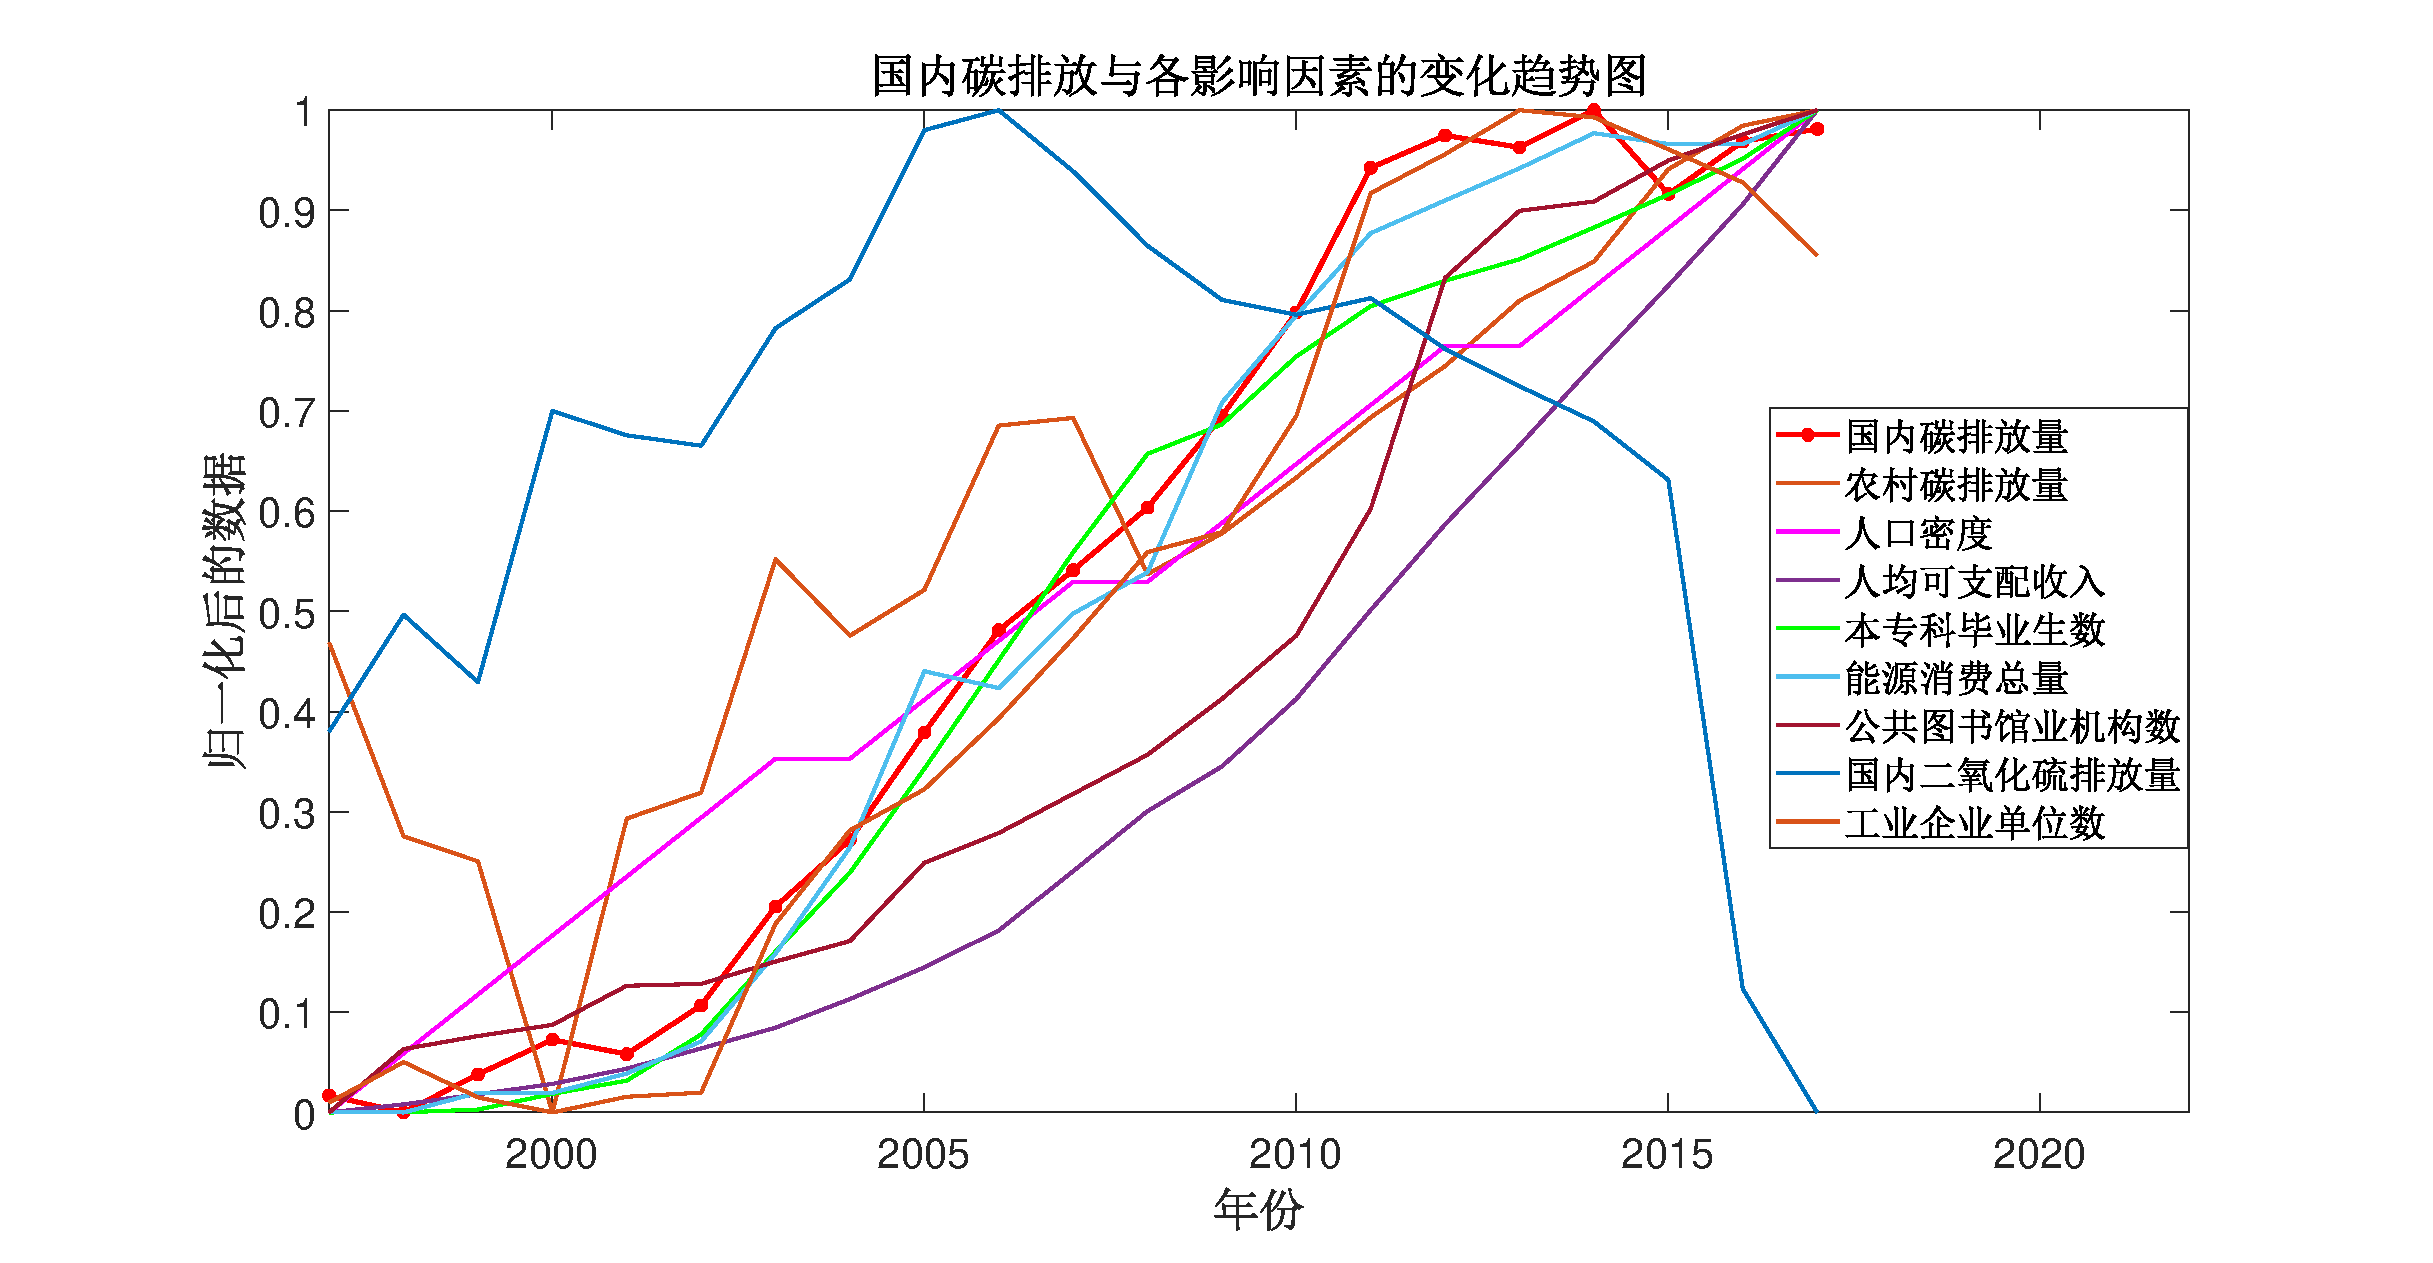
\includegraphics[width=0.7\linewidth]{China_trend.eps}
	\caption{1997-2017国内碳排放与各影响因素变化趋势图}
	\label{fig:chinatrend}
\end{figure}

	分析图\ref{fig:chinatrend},发现国内二氧化硫排放量折线与国内碳排放量折线差异最大,故初步推断国内二氧化硫排放量可能不是影响国内碳排放量的主要影响因素,而选出的其他影响因素是否是国内碳排放量的主要影响因素难以由趋势图\ref{fig:chinatrend}来判断,需要进一步的模型去进行判断。
	
\subsection{基于Pearson相关性分析进行特征选择}
基于问题一、二所建模型,本文通过式\eqref{eq:9}计算了国内碳排放量与所选取的各影响因素间的Pearson相关系数,并经过$t$检验后来判断国内碳排放量的主要影响因素有哪些。
\begin{equation}
	\label{eq:9}
	{{C}_{p}}(a,b)=\frac{cov(a,b)}{{{\sigma }_{a}}{{\sigma }_{b}}}=\frac{\sum_{i}^{N}{({{a}_{i}}-\bar{a})({{b}_{i}}-\bar{b})}}{\sqrt{\sum_{i}^{N}{{{({{a}_{i}}-\bar{a})}^{2}}}}\sqrt{\sum_{i}^{N}{{{({{b}_{i}}-\bar{b})}^{2}}}}}
\end{equation}

计算结果为:
\begin{align*}
	{C_p}(China\_Carbon,Countryside\_Carbon)=0.8804
\end{align*}
\begin{align*}
	{C_p}(China\_Carbon,population\_density)=0.9661
\end{align*}
\begin{align*}
	{C_p}(China\_Carbon,income)=0.9233
\end{align*}
\begin{align*}
	{C_p}(China\_Carbon,graduate)=0.9915
\end{align*}
\begin{align*}
	{C_p}(China\_Carbon,energy)=0.9170
\end{align*}
\begin{align*}
	{C_p}(China\_Carbon,library)=0.9417
\end{align*}
\begin{align*}
	{C_p}(China\_Carbon,SO_2)=-0.0728
\end{align*}
\begin{align*}
	{C_p}(China\_Carbon,enterprise)=0.9915
\end{align*}


	其中,$China\_Carbon$表示全球碳排放量,$Countryside\_Carbon$表示农村碳排放量,$population\_density$表示人口密度,$income$表示人均可支配收入,$graduate$表示本科专科毕业生数,$energy$表示能源消费总量,$library$表示公共图书馆业机构,$SO_2$表示国内二氧化硫排放量,$enterprise$表示工业企业单位数。将所得Pearson相关系数绘制成由颜色深浅显示两个变量间相关性的热力图如图\ref{fig:corrchina}所示:
	
% TODO: \usepackage{graphicx} required
\begin{figure}[htbp]
	\centering
	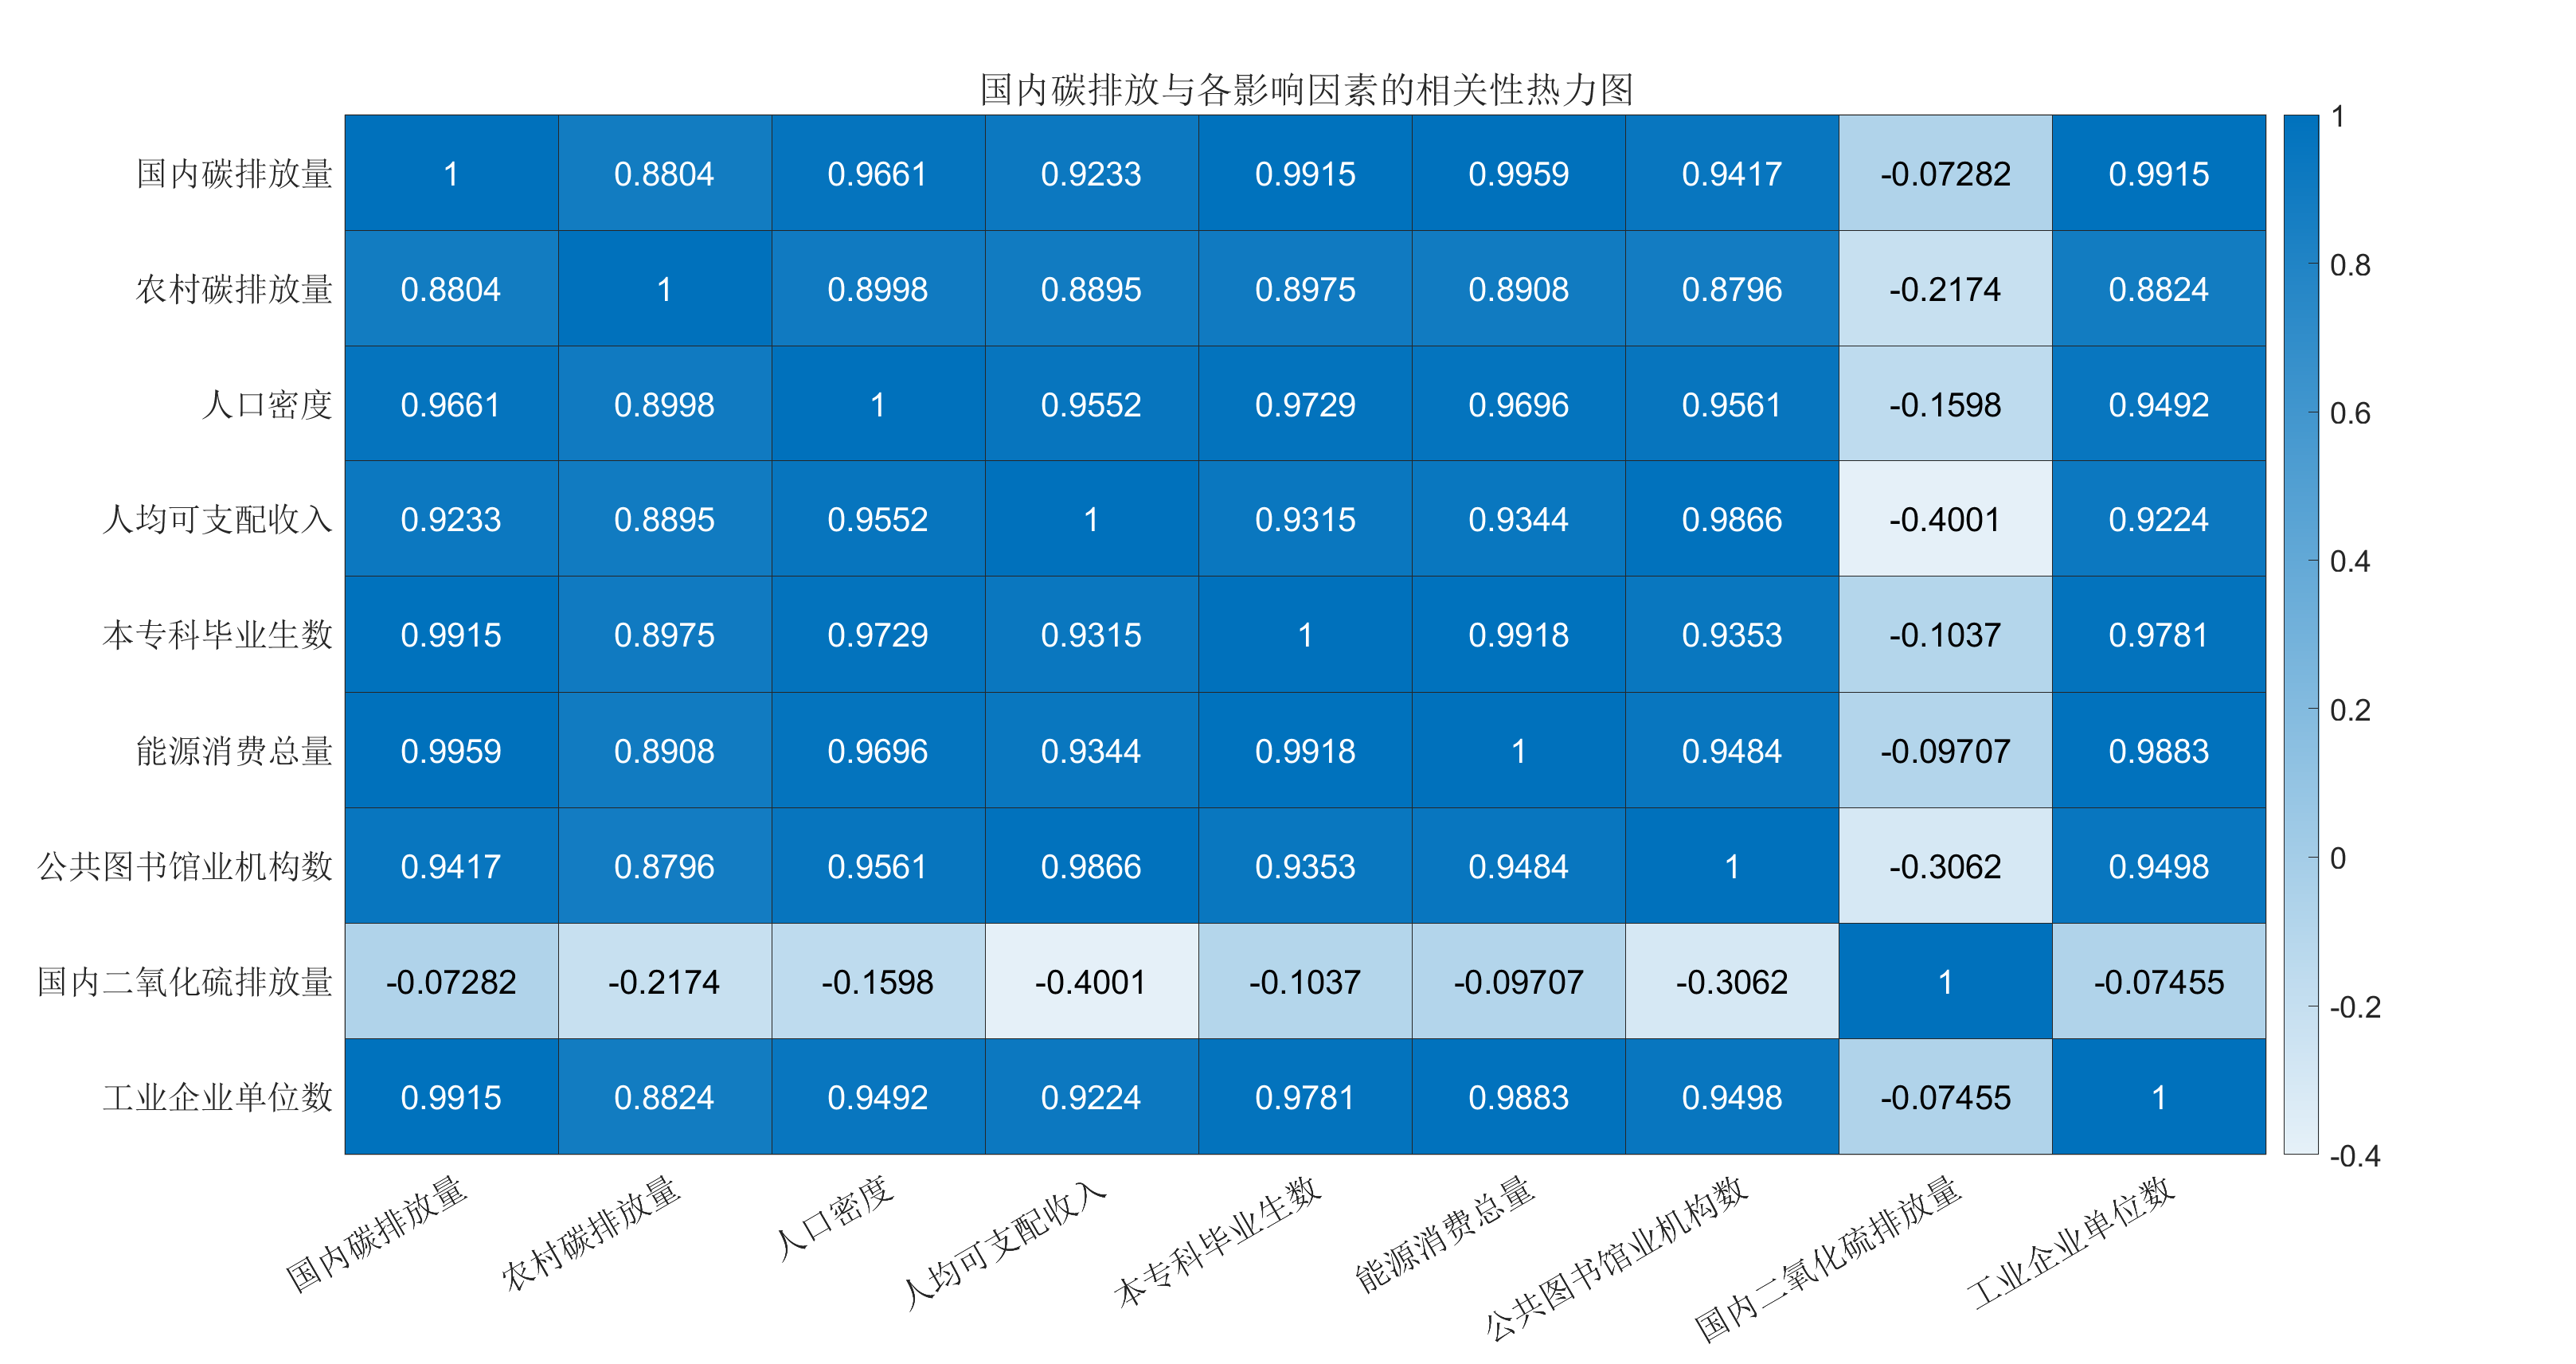
\includegraphics[width=0.9\linewidth]{corr_china.eps}
	\caption{国内碳排放与各影响因素的相关性热力图}
	\label{fig:corrchina}
\end{figure}
	

可以提取热力图与国内碳排放量相关的数据,简化为更直观的直方图如图 \ref{fig:corrdecent}所示。
	
% TODO: \usepackage{graphicx} required
\begin{figure}[H]
	\centering
	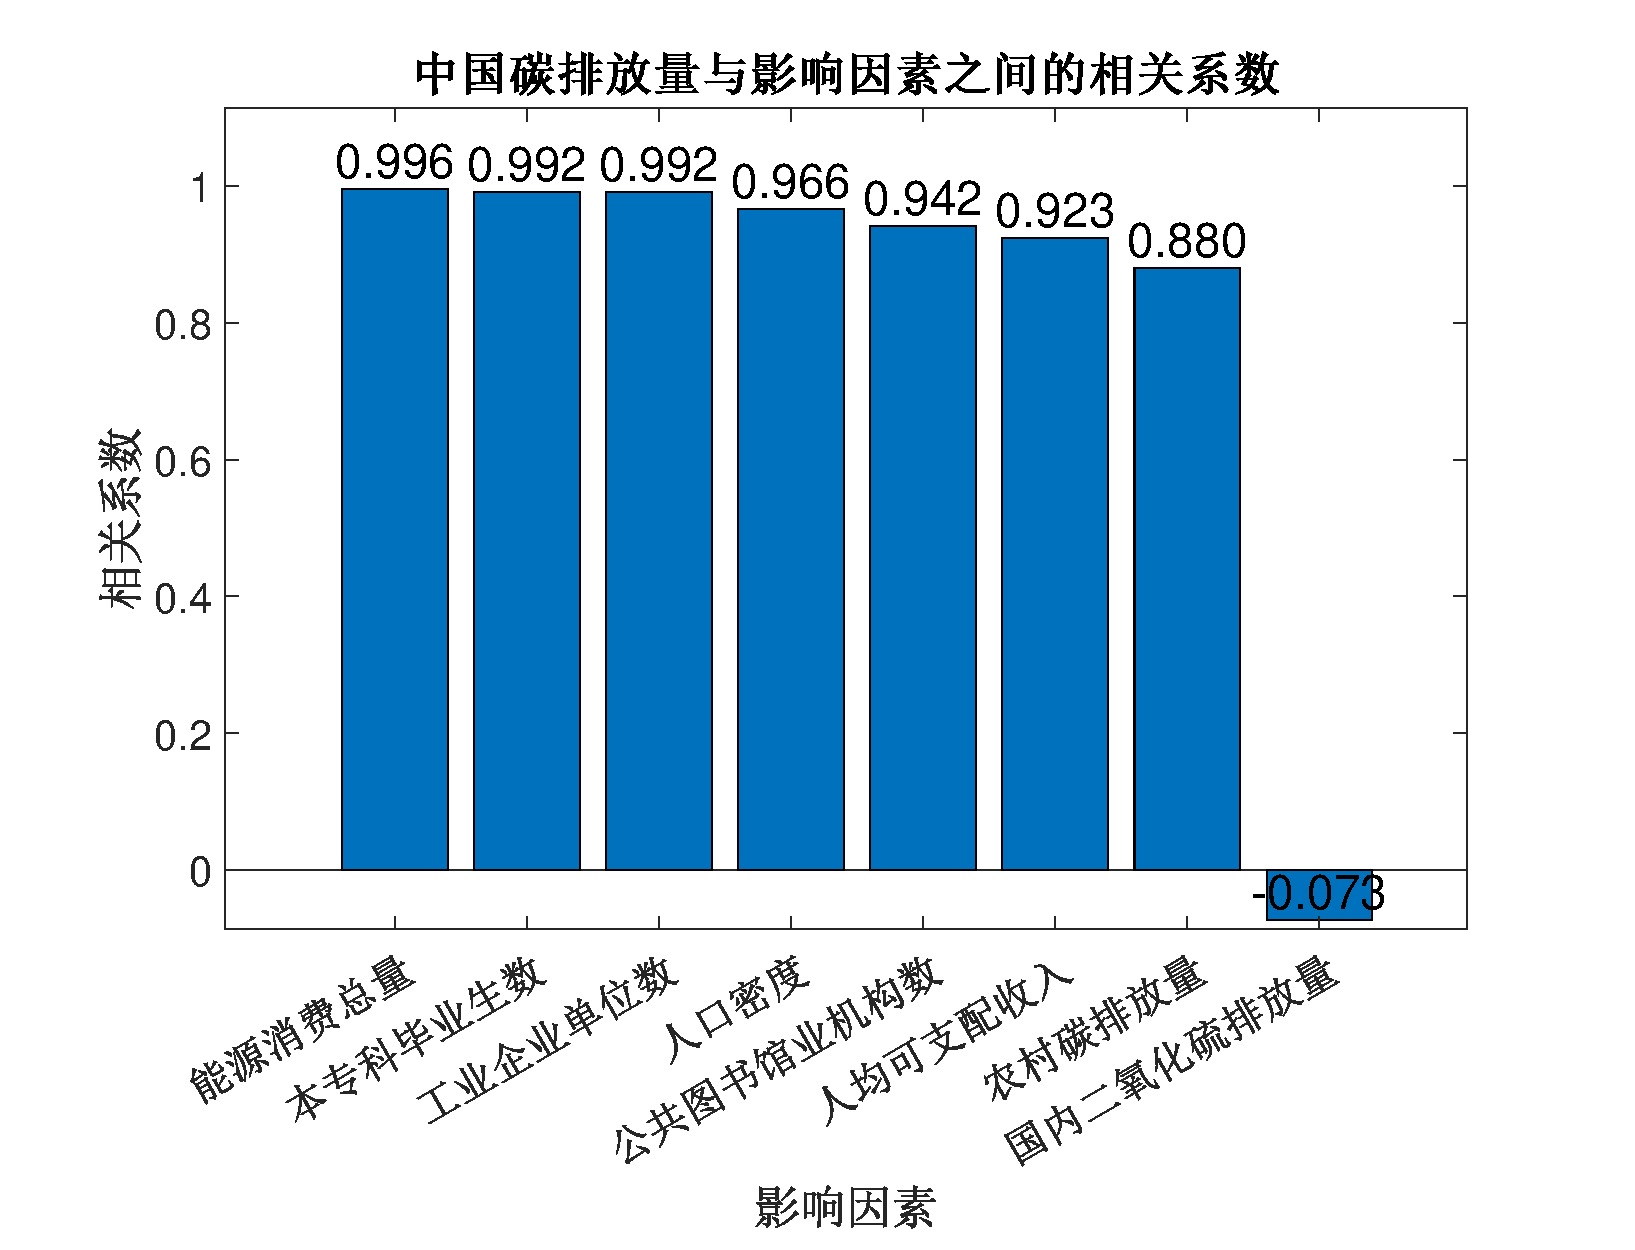
\includegraphics[width=0.9\linewidth]{corr_decent.eps}
	\caption{简化后相关系数直方图}
	\label{fig:corrdecent}
\end{figure}

	由图不难看出,国内二氧化硫的排放量与国内碳排放量的相关系数的绝对值最低,两者相关性最弱,其余所选取的影响因素与国内碳排放量的相关性较强。但对计算所得的相关系数的合理性,仍需进行假设检验。
	
	设置零假设$H_0$:相关性系数为0,即选取的各影响因素各自与国内碳排放量间都五显著的相关性与备择假设$H_{1}$ :相关性系数不为0,即每两个变量之间存在显著的线性相关关系。由式\eqref{eq:10}计算各组相关系数的$t$ 统计量:
	\begin{equation}
		\label{eq:10}
		t={{C}_{p}}(a,b)\sqrt{\frac{N-2}{1-{{\left [{{{C}_{p}}(a,b)}\right ]}^{2}}}}
	\end{equation}
	
	计算后得到:
	\begin{align*}
		p(China\_Carbon,Countryside\_Carbon)=0<\alpha
	\end{align*}
	\begin{align*}
		p(China\_Carbon,population\_density)=0<\alpha
	\end{align*}
	\begin{align*}
		p(China\_Carbon,income)=0<\alpha
	\end{align*}
	\begin{align*}
		p(China\_Carbon,graduate)=0<\alpha
	\end{align*}
	\begin{align*}
		p(China\_Carbon,energy)=0<\alpha
	\end{align*}
	\begin{align*}
		p(China\_Carbon,library)=0<\alpha
	\end{align*}
	\begin{align*}
		p(China\_Carbon,SO_2)=0.7538>\alpha
	\end{align*}
	\begin{align*}
		p(China\_Carbon,enterprise)=0<\alpha
	\end{align*}
	故假设检验结果为:除$SO_2$接受零假设外,其余所选取的影响因素均拒绝原假设,即可以判断国内二氧化硫排放量不是国内碳排放量的主要影响因素。
	
	故对于国内碳排放量的主要影响因素进行特征选择,得主要影响因素有农村碳排放量,人口密度,人均可支配收入,本科专科毕业生数,能源消费总量,公共图书馆业机构,工业企业单位数7个特征变量。
	
	\subsection{基于随机森林模型的多元回归}
	\subsubsection{随机森林的多元回归模型的建立}
	随机森林模型的实质是一个包含多个决策树的回归器,这些决策树的形成采用了随机的方法,因此也叫做随机决策树,决策树之间是没有关联,当测试数据进入随机森林时,每棵决策树对数据进行回归,最终取所有决策树中回归结果最多的一类作为最终输出的结果。将同一年的国内碳排放量及其7个主要影响因素数据作为一个样本点,设样本的属性个数为$R$,$r \in {Z^ + },0<r<R$,由于本体样本点较少,随机森林重采样的输出结果质量较差,故本文采用贝叶斯算法对随机森林的超参数进行优化,以得到最优的超参数组合,提高随机森林模型的性能表现
	
	将国内碳排放量作为响应变量,7个主要影响因素:农村碳排放量,人口密度,人均可支配收入,本科专科毕业生数,能源消费总量,公共图书馆业机构,工业企业单位数作为预测变量。
	
	在构建决策树前,本文首先通过主成分分析(PCA)的方法,对数据进行降维处理,得出各影响因素的累积贡献率的直方图如图\ref{fig:pca}所示:
	
\begin{figure}[htbp]
	\centering
	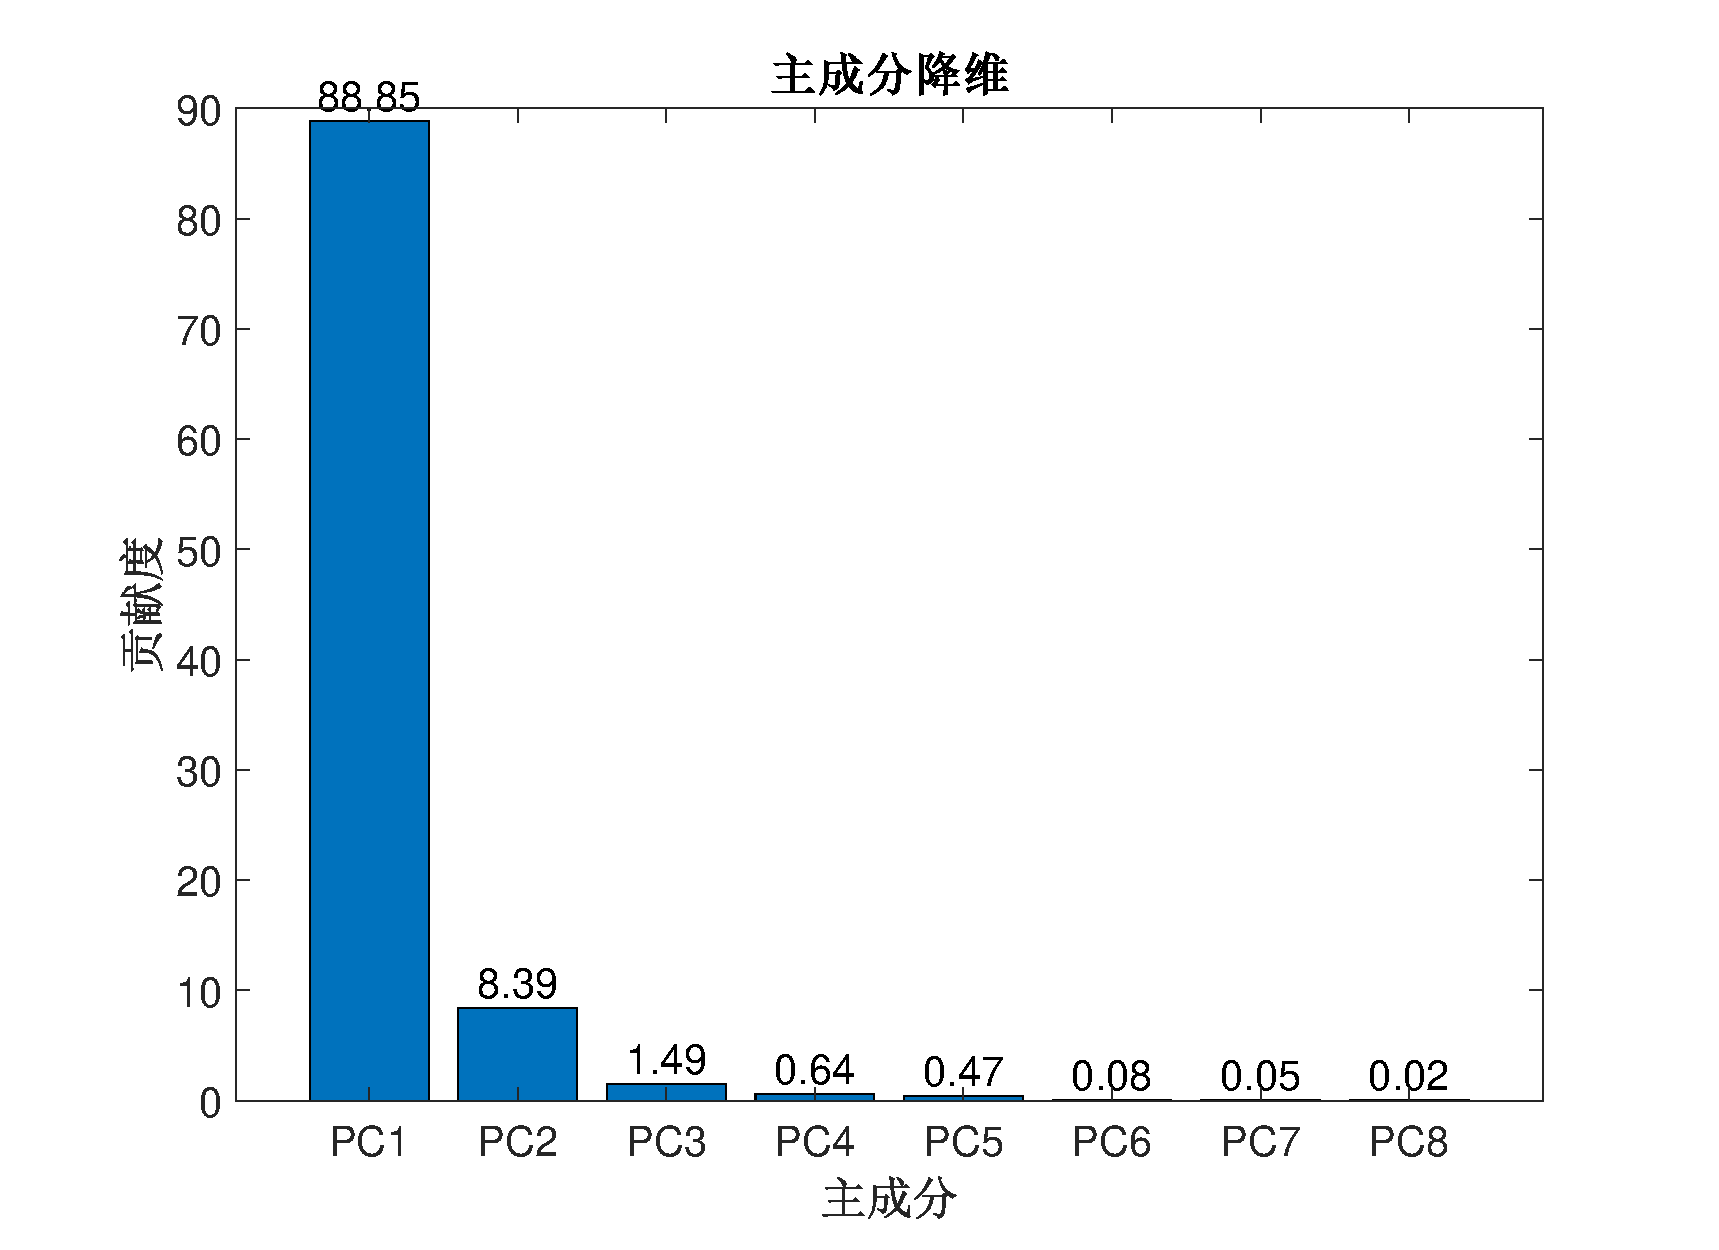
\includegraphics[width=0.65\linewidth]{PCA.eps}
	\caption{主成分贡献率直方图}
	\label{fig:pca}
\end{figure}

由于PCA模型仅保留足以解释95\%方差的成分,在训练后,主成分减少为两个,由于主成分分析后损失的信息较多,故本文随机森林模型同时进行PCA分析和不进行PCA分析两种方法进行回归训练。


\subsubsection{随机森林的多元回归模型的预测结果}

分别进行有PCA和无PCA的随机森林回归训练,计算模型中平均预测误差的平方根$RMSE$、平方$MSE$、绝对值$MAE$和决定系数$R^2$,得到的两种评估指标数据如下表:

\begin{table}[htb]
	\centering
	\begin{tabular}{ccccc} 
		\hline
		模型   & $RMSE$        &$ MSE$         & $R^2 $     &$ MAE$          \\ 
		\hline
		随机森林(有PCA) & 0.082822263 & 0.006859527 & 0.954972247 & 0.065432281  \\
		\textbf{随机森林(无PCA)} &\textbf{ 0.083441865} &\textbf{ 0.006962545} & \textbf{0.954296011} & \textbf{0.070921787}  \\
		\hline
	\end{tabular}
\end{table}

分析对比表可以得知,无PCA的随机森林回归模型的预测性能更好,拟合效果更优,预测值和实际值之间的偏差更小。故采用无PCA降维的随机森林回归模型,预测国内碳排放量的结果如下图\ref{fig:randomforestmodelpredict1997-2017}所示:
% TODO: \usepackage{graphicx} required
\begin{figure}[htb]
	\centering
	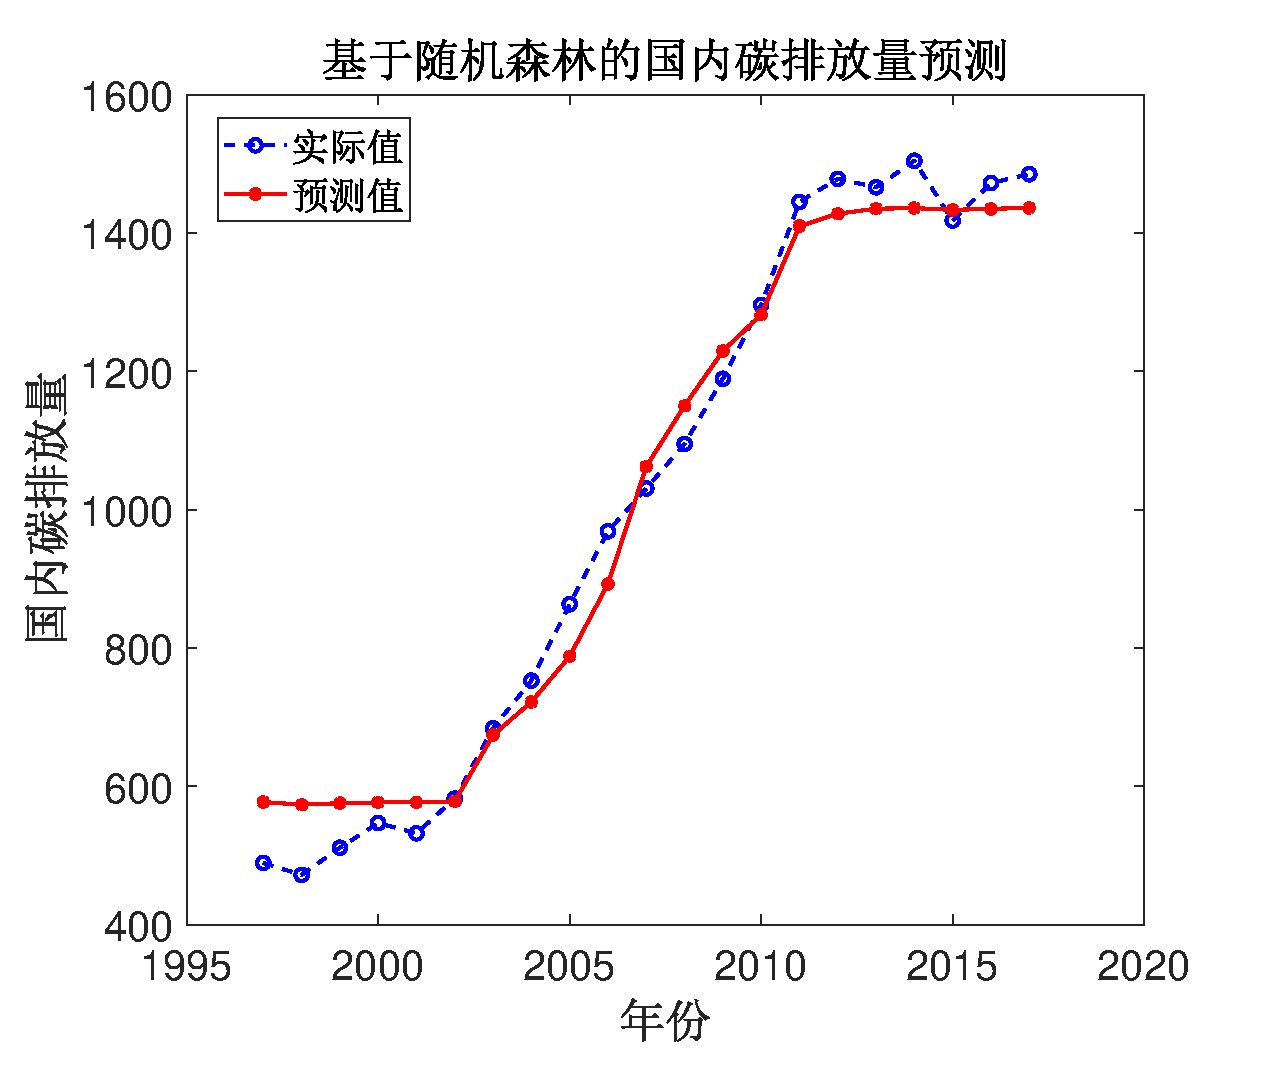
\includegraphics[width=0.7\linewidth]{figures/pro3/random_forest_model_predict1997-2017}
	\caption{随机森林预测结果}
	\label{fig:randomforestmodelpredict1997-2017}
\end{figure}

可见预测值的趋势与实际值的趋势基本吻合。

\subsection{基于LSTM的时间序列预测}

由于预测变量与响应变量都是时间序列,具有明显的趋势性,故本文采用时间序列预测模型预测7个预测变量从2018到2032年的值。首先采用 ARIMA、岭回归、灰色预测模型等统计时间序列模型进行预测,结果发现效果较差。因此本文采用 LSTM 长短时记忆网络模型进行预测。
\subsubsection{LSTM模型}
    LSTM(Long short-term memory 长短期记忆网络)通过细胞状态和门控机制来管理控制信息的流动,使其能够有效地捕捉时间序列数据中的长期依赖关系,是一种强大的时间序列预测工具。主要优点可以概括为:
    
	• \textbf{长期记忆能力}:引入“细胞状态”内部状态,捕捉和保留序列中的长期依赖关系;
	
 	• \textbf{门控机制}:遗忘门、输入门和输出门这些门控单元通过学习来控制信息的流动,有效地管理细胞状态的更新和选择性遗忘;
 	
    • \textbf{反向传播稳定性}:由于 LSTM 的门控机制,它在反向传播时通常不会出现梯度消失或爆炸的问题,训练更加容易。
    
  \iffalse  



	将预测变量代入LSTM模型得出结果后,对模型的性能进行进行诊断,提取随机森林回归时有无PCA分析在LSTM预测后的输出结果,计算模型中平均预测误差的平方根$RMSE$、平方$MSE$、绝对值$MAE$和决定系数$R^2$,得到的两种评估指标数据如下表:
	
	\begin{table}[htbp]
		\centering
		\begin{tabular}{ccccc} 
			\hline
			模型   & RMSE        & MSE         & $R\^{}2$      & MAE          \\ 
			\hline
			$p_0$ & 0.082822263 & 0.006859527 & 0.954972247 & 0.065432281  \\
			$p_1$ & 0.083441865 & 0.006962545 & 0.954296011 & 0.070921787  \\
			\hline
		\end{tabular}
			\end{table}
		
		分析对比表可以得知,在随机森林回归时不进行PCA的LSTM预测模型性能更好,拟合效果更优,预测值和实际值之间的偏差更小。在随机森林回归时不进行PCA的LSTM预测模型下得到各预测变量的预测图如下:能源消费总量、本专科毕业生数、工业企业单位数、人口密度、公共图书馆业机构数、人均可支配收入、农村碳排放量、国内二氧化硫排放量
\fi		
\subsubsection{将预测变量代入LSTM模型}
搭建 LSTM 模型对7个预测变量:农村碳排放量,人口密度,人均可支配收入,本科专科毕业生数,能源消费总量,公共图书馆业机构,工业企业单位数作进行时间序列预测,LSTM 模型参数如下:
\begin{table}[htb]
	\centering
	\caption{LSTM 模型参数}
	\begin{tabular}{cc|cc} 
		\hline
		单层 LSTM单元数 & 6   & 损失函数~ & 均方误差   \\
		全连接层神经元数   & 7   & 优化器~  & Adam  \\
		迭代次数       & 300 & 样本批量 & 7      \\
		\hline
	\end{tabular}
\end{table}

7个预测变量的在2018-2032年的预测结果如下图所示:

\begin{figure}[h]
	\begin{minipage}{0.32\linewidth}
		\centerline{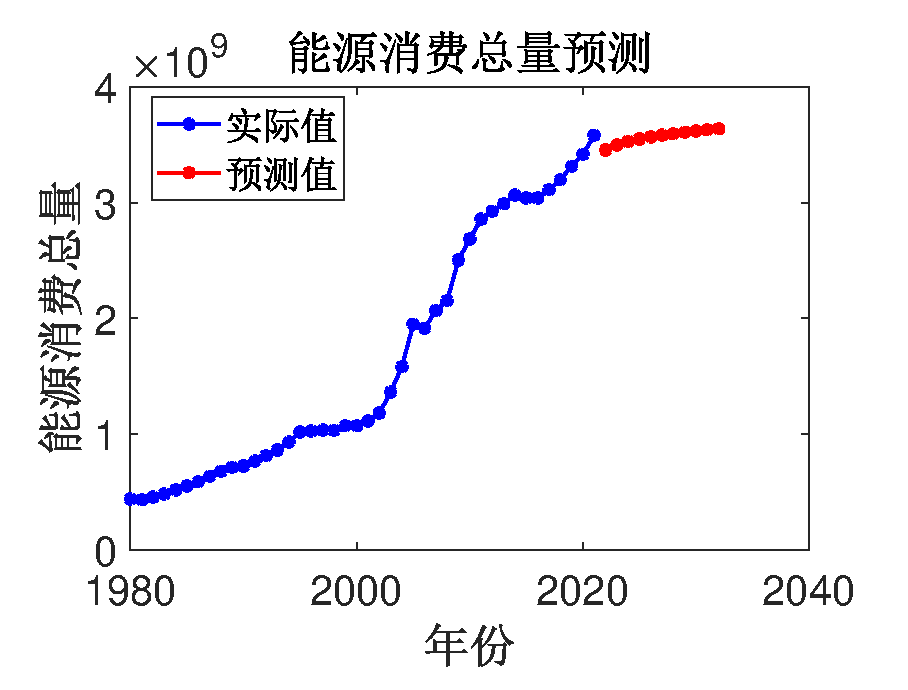
\includegraphics[width=\textwidth]{energy_predict.eps}}
	\end{minipage}
	\begin{minipage}{0.32\linewidth}
		\centerline{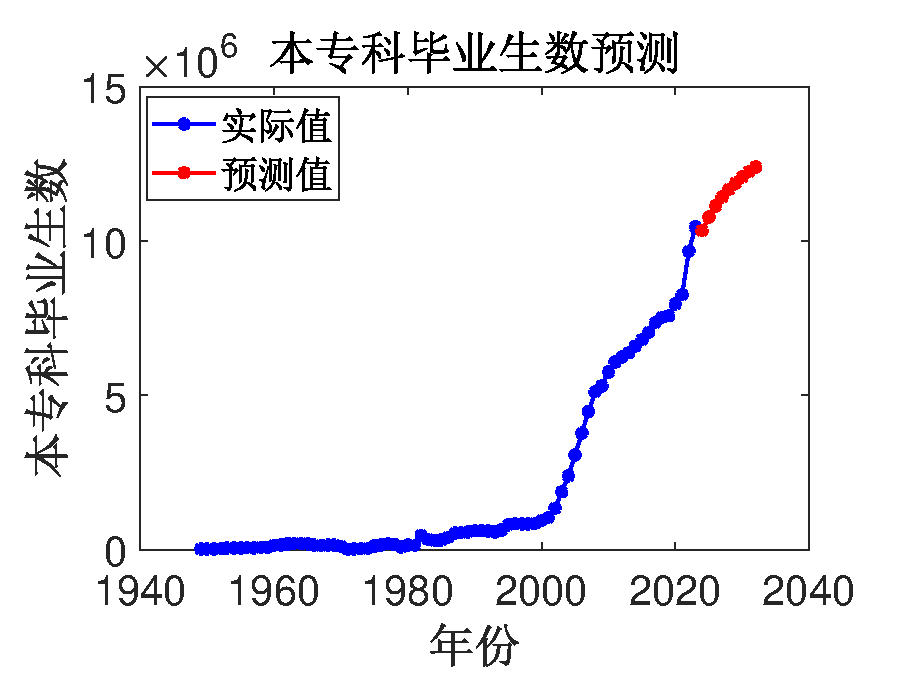
\includegraphics[width=\textwidth]{graduate_predict.eps}}
	\end{minipage}
	\begin{minipage}{0.32\linewidth}
		\centerline{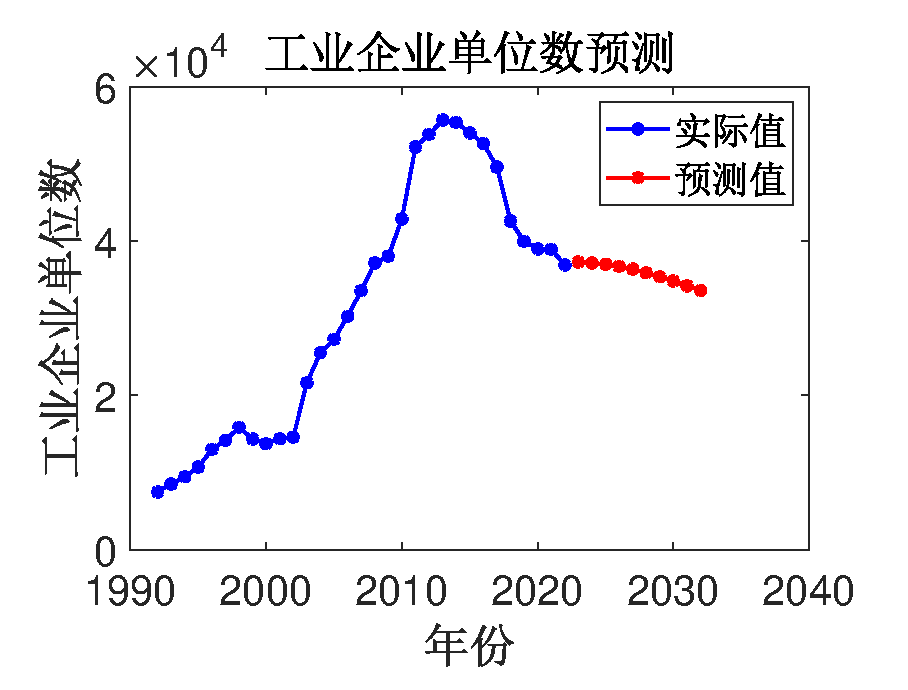
\includegraphics[width=\textwidth]{enterprise_predict.eps}}
	\end{minipage}
	\label{fig:images}
\end{figure}

\begin{figure}[htbp]
	\centering
	\subcaptionbox{\label{fig:图d1}}
	{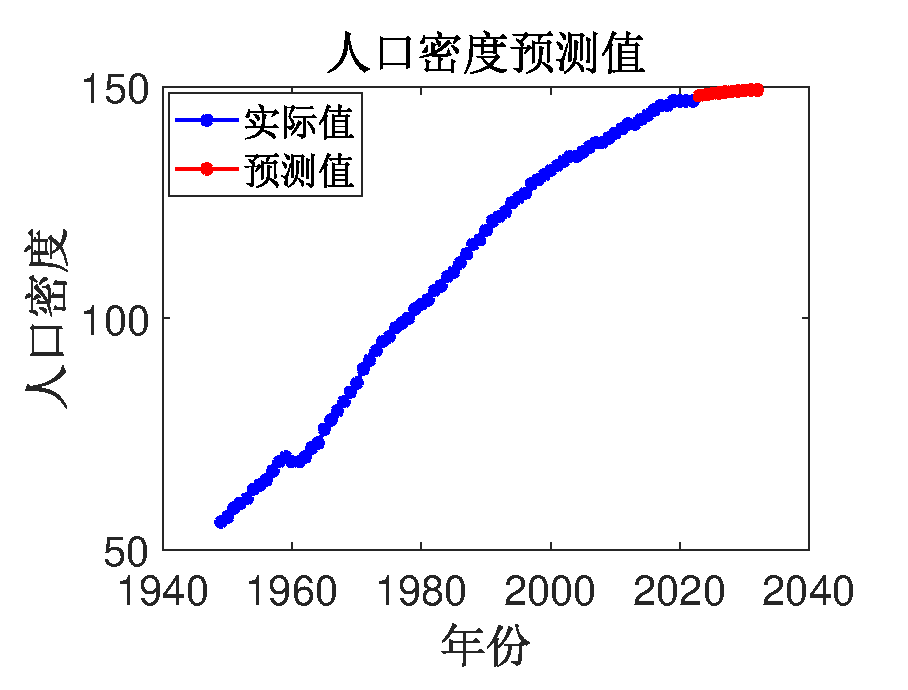
\includegraphics[width=.4\textwidth]{density_predict.eps}}
	\subcaptionbox{\label{fig:图d2}}
	{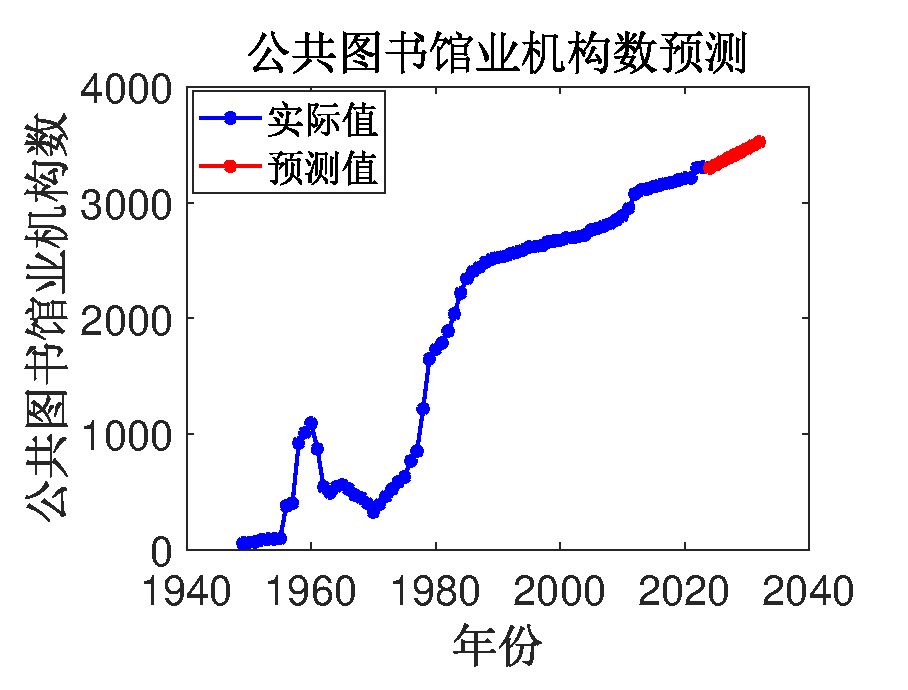
\includegraphics[width=.4\textwidth]{lib_predict.eps}}
	\subcaptionbox{\label{fig:图d3}}
	{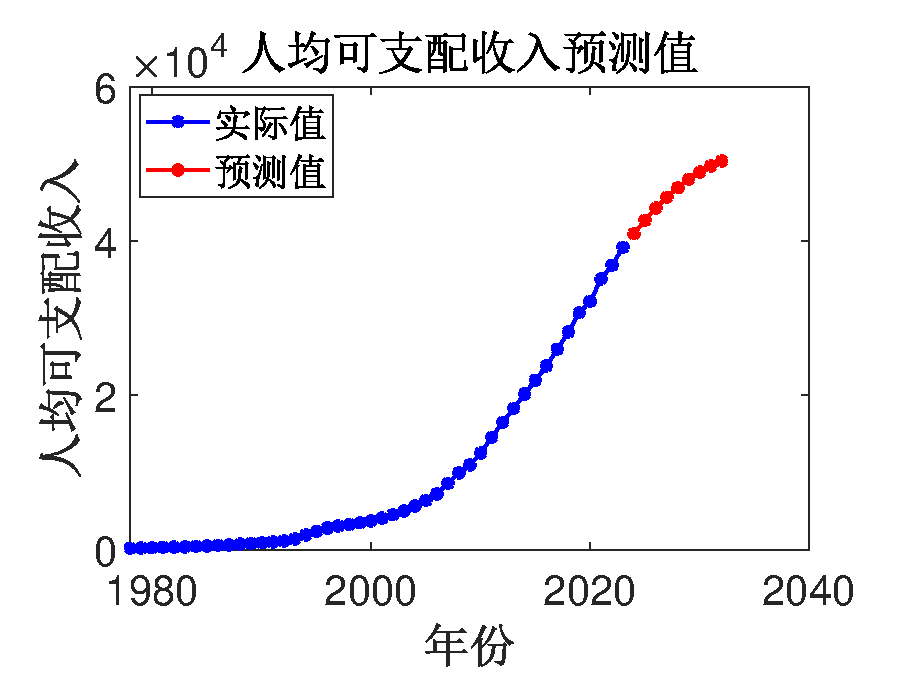
\includegraphics[width=.4\textwidth]{income_predict.eps}}
	\subcaptionbox{\label{fig:图d4}}
	{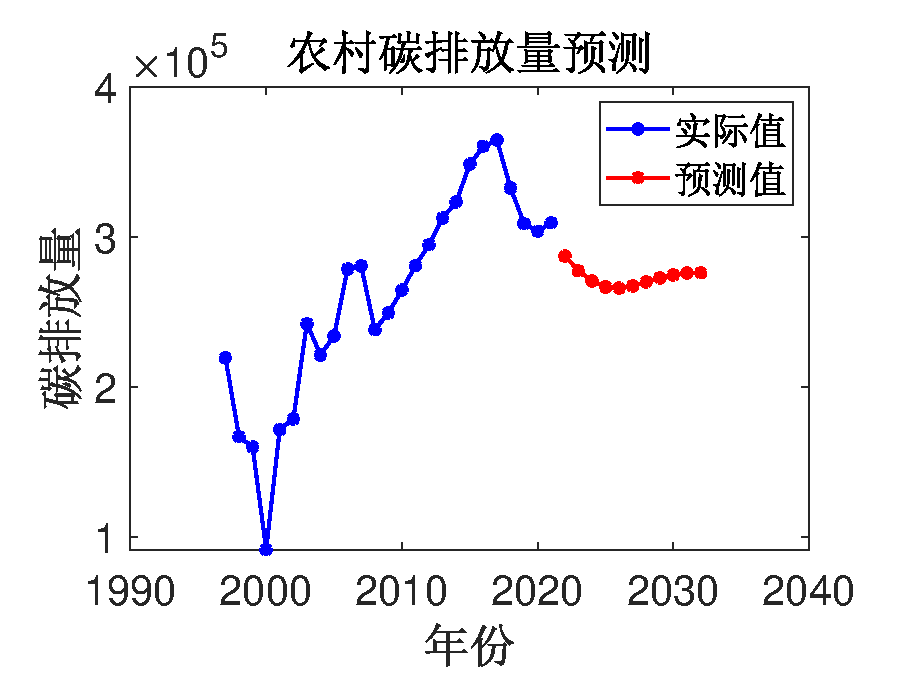
\includegraphics[width=.4\textwidth]{countryside_predict.eps}}
	\label{fig:四图}
\end{figure}

	\subsection{基于随机森林模型预测未来碳排放量}
将LSTM预测模型得到各预测变量在2018-2032年的预测值代入随机森林的回归模型中,可得国内碳排放量的在2018-2032年预测值,国内碳排放的预测图如下:

% TODO: \usepackage{graphicx} required
\begin{figure}[htb]
	\centering
	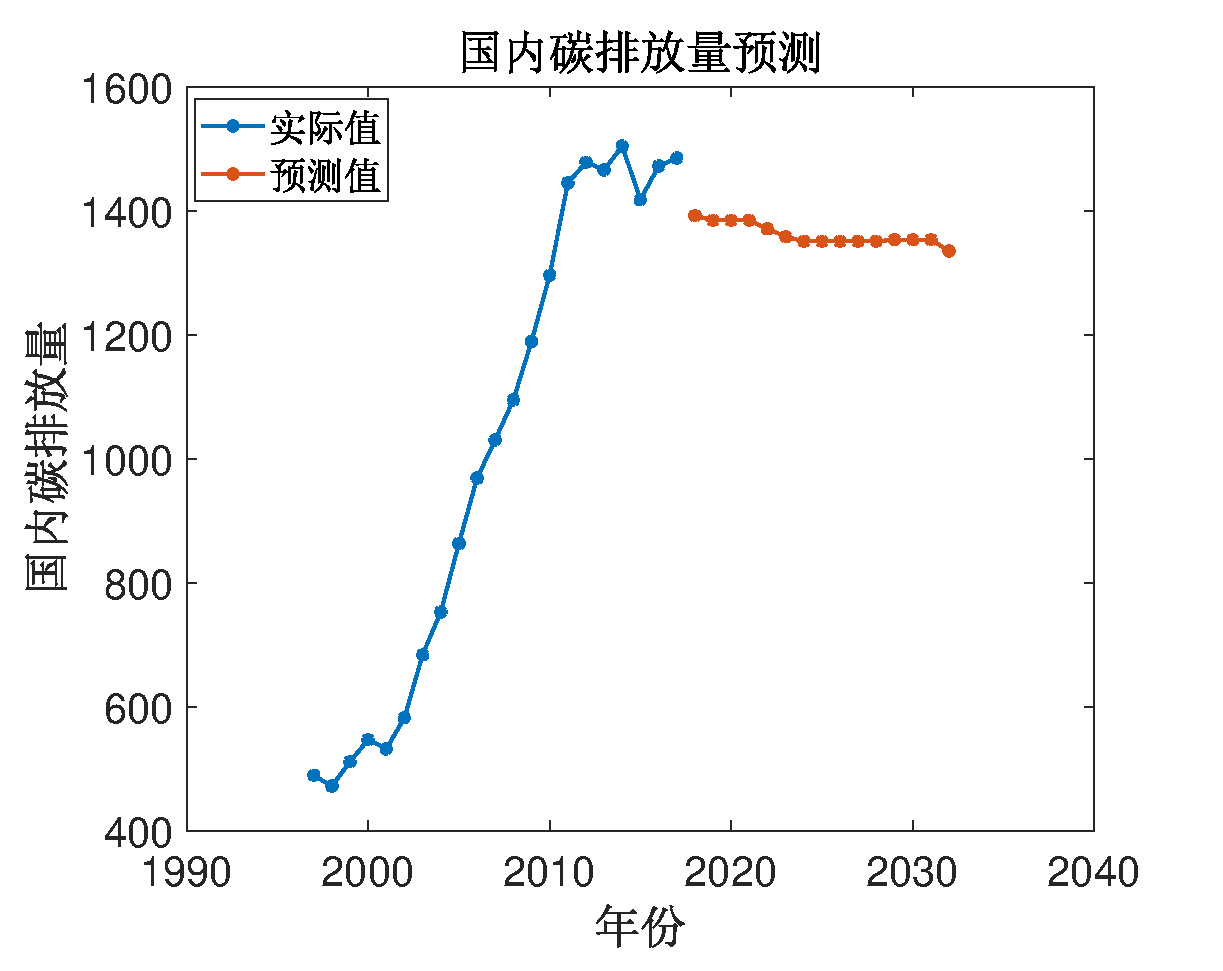
\includegraphics[width=0.7\linewidth]{random_forest_predict2018-2032.eps}
	\label{fig:randomforestpredict2018-2032}
\end{figure}

分析上图可知,国内碳排放量在2018年后开始逐渐、缓慢下降,故可推断2030年达到碳达峰的目标可行。


	

%%%%%%%%%%%%%%%%%%%%%%%%%%%%%%%%%%%%%%%%%%%%%%%%%%%%%%%%%%%%% 

\section{问题四的模型的建立和求解}
随着全球气候变化和环境问题日益严重,减少碳排放已成为国际社会共同关注的重要议题。人工智能技术作为21世纪最具创新性和影响力的技术之一,在科技减碳方面展现出巨大的潜力和价值。本文将从优化能源结构、提高能效、智能交通系统、建筑智能化、精准农业技术、碳捕捉和存储技术(CCS)以及智能数据分析和监测等方面,探讨人工智能技术在科技减碳方面的建议。

\subsection{优化能源结构}
人工智能技术可以通过数据分析和预测模型,为能源结构的优化提供科学依据。例如,通过对不同能源类型的产能、消耗、碳排放等因素的综合评估,为政策制定者提供决策支持,推动清洁能源如太阳能、风能等的大规模开发和利用。此外,人工智能技术还可以优化能源分配和调度,提高能源利用效率,降低碳排放。

\subsection{提高能效}
在工业生产和日常生活中,人工智能技术可以通过智能调度、优化生产流程、改进设备运行状态等方式,实现能效的提高。例如,智能制造系统可以收集和分析生产数据,实现智能调度和优化,减少不必要的能源消耗。同时,人工智能技术还可以应用于智能能源管理,实时监控能源消耗情况,优化能源配置,减少能源浪费。

\subsection{智能交通系统}
智能交通系统是人工智能技术在交通领域的重要应用之一。通过智能交通管控系统,可以实现对交通流量的优化控制,减少交通拥堵,提高交通效率,从而减少交通排放。此外,人工智能技术还可以加速电动汽车充电站的建设与管理,推动电动交通的发展,进一步减少碳排放。

\subsection{建筑智能化}
在建筑领域,人工智能技术可以通过建筑模拟和能源消耗模型的分析,帮助设计师和规划者优化建筑设计和城市布局,实现更加节能和环保的建筑和城市。同时,人工智能技术还可以通过智能控制系统,实现建筑内部能源的智能管理,降低能源消耗,减少碳排放。

\subsection{精准农业技术}
精准农业技术通过人工智能驱动的工具提供作物管理、灌溉调度和病虫害防治方面的见解,实现更可持续、更环保的农业实践。人工智能技术可以根据土壤、气候和作物生长情况,制定科学的种植方案,减少化肥和农药的使用,降低农业生产过程中的碳排放。

\subsection{碳捕捉和存储技术(CCS)}
人工智能技术可以优化碳捕获和储存流程,提高CCS技术的效率和可行性。通过机器学习算法,可以分析与CCS操作相关的大量数据集,提高在碳排放进入大气之前捕获碳排放的整体效率和可行性。这将有助于实现工业过程中的大规模减碳,为应对气候变化提供重要支持。

\subsection{智能数据分析和监测}
智能数据分析和监测是实现科技减碳的重要手段之一。通过实施人工智能监测系统,可以持续跟踪和报告各个行业的碳排放情况。实时数据分析和报告机制使组织和政府能够评估其环境影响,并采取积极措施减少排放。此外,人工智能还可以通过分析历史数据和预测模型,为减碳政策的制定和实施提供科学依据。

\subsection{结论:}
人工智能技术在科技减碳方面具有广泛的应用前景和巨大的潜力。通过优化能源结构、提高能效、智能交通系统、建筑智能化、精准农业技术、碳捕捉和存储技术(CCS)以及智能数据分析和监测等手段的综合运用,可以有效降低碳排放,推动全球绿色低碳发展。未来,随着人工智能技术的不断发展和完善,其在科技减碳方面的作用将更加显著和重要。

%%%%%%%%%%%%%%%%%%%%%%%%%%%%%%%%%%%%%%%%%%%%%%%%%%%%%%%%%%%%%

\section{模型的评价}

\subsection{模型的优点}
\begin{itemize}[itemindent=2em]
\item 优点1:Pearson相关性分析简单易懂,表达直观,可解释性强。
\item 优点2:随机森林对于数据中的噪声和缺失值具有很强的鲁棒性,能够处理复杂的数据集,准确性高,训练速度快,且不容易过拟合。
\item 优点3:LSTM模型可以用于处理各种类型的时间序列数据,包括具有复杂模式和非线性关系的数据,且通常能够实现较高的预测准确性。
\end{itemize}

\subsection{模型的缺点}
\begin{itemize}[itemindent=2em]
\item 缺点1:Pearson相关性分析只能检测到线性关系,对于非线性关系的相关性无法很好地反映,且要求变量符合正态分布,如果数据不符合正态分布,则相关性分析结果可能不准确。
\item 缺点2:随机森林是一种黑盒模型,难以解释为什么会做出特定的预测。
\item 缺点3:LSTM模型在处理小型数据集或数据噪声较大的情况下,可能存在过拟合的风险,需要采取适当的正则化方法。并且LSTM模型有许多超参数需要调优,如网络结构、学习速率等,不当的选择可能会影响模型的性能。
\end{itemize}

\newpage
%%%%%%%%%%%%%%%%%%%%%%%%%%%%%%%%%%%%%%%%%%%%%%%%%%%%%%%%%%%%%
%% 参考文献
\nocite{*}
\bibliographystyle{gbt7714-numerical}  % 引用格式
\bibliography{ref.bib}  % bib源

\newpage
%%%%%%%%%%%%%%%%%%%%%%%%%%%%%%%%%%%%%%%%%%%%%%%%%%%%%%%%%%%%%
%% 附录
\begin{appendices}
\section{文件列表}
\begin{table}[H]
\centering
\begin{tabularx}{\textwidth}{LL}
\toprule
文件名   & 功能描述 \\
\midrule
pro1.m & 问题一程序代码 \\
pro2.m & 问题二程序代码 \\
pro3.m & 问题三程序代码 \\
LSTM.m & LSTM模型代码 \\
\bottomrule
\end{tabularx}
\label{tab:文件列表}
\end{table}

\section{代码}
\noindent pro1.m
\lstinputlisting[language=matlab]{code/pro1.m}
pro2.m
\lstinputlisting[language=matlab]{code/pro2.m}
pro3.m
\lstinputlisting[language=matlab]{code/pro3.m}
LSTM.m
\lstinputlisting[language=matlab]{code/LSTM.m}
\end{appendices}
\end{document}




\section{表格}



\begin{table}
	\centering
	\caption{中国碳排放量与影响因素之间的相关系数矩阵}
	\begin{tabular}{c|cccccccccc} 
		\cline{1-10}
		& China\_Carbon & Countryside\_Carbon & population\_density & income  & graduate & energy  & library & SO2     & enterprise & enterprise  \\ 
		\cline{1-10}
		China\_Carbon       & 1.0000        & 0.8804              & 0.9661              & 0.9233  & 0.9915   & 0.9170  & 0.9417  & -0.0728 & 0.9915     &             \\
		Countryside\_Carbon & 0.8804        & 1.0000              & 0.8998              & 0.8895  & 0.8975   & 0.9104  & 0.8796  & -0.2174 & 0.8824     &             \\
		population\_density & 0.9661        & 0.8998              & 1.0000              & 0.9552  & 0.9729   & 0.8821  & 0.9561  & -0.1598 & 0.9492     &             \\
		income              & 0.9233        & 0.8895              & 0.9552              & 1.0000  & 0.9315   & 0.9077  & 0.9866  & -0.4001 & 0.9224     &             \\
		graduate            & 0.9915        & 0.8975              & 0.9729              & 0.9315  & 1.0000   & 0.9209  & 0.9353  & -0.1037 & 0.9781     &             \\
		energy              & 0.9170        & 0.9104              & 0.8821              & 0.9077  & 0.9209   & 1.0000  & 0.9032  & -0.2421 & 0.9221     &             \\
		library             & 0.9417        & 0.8796              & 0.9561              & 0.9866  & 0.9353   & 0.9032  & 1.0000  & -0.3062 & 0.9498     &             \\
		SO2                 & -0.0728       & -0.2174             & -0.1598             & -0.4001 & -0.1037  & -0.2421 & -0.3062 & 1.0000  & -0.0745    &             \\
		enterprise          & 0.9915        & 0.8824              & 0.9492              & 0.9224  & 0.9781   & 0.9221  & 0.9498  & -0.0745 & 1.0000     &             \\
		\cline{1-10}
	\end{tabular}
\end{table}

\begin{table}
	\centering
	\caption{中国碳排放量与影响因素之间的相关系数矩阵p值}
	\begin{tabular}{c|ccccccccc} 
		\hline
		& China\_Carbon & Countryside\_Carbon & population\_density & income & graduate & energy & library & SO2    & enterprise  \\ 
		\hline
		China\_Carbon       & 1.0000        & 0.0000              & 0.0000              & 0.0000 & 0.0000   & 0.0000 & 0.0000  & 0.7538 & 0.0000      \\
		Countryside\_Carbon & 0.0000        & 1.0000              & 0.0000              & 0.0000 & 0.0000   & 0.0000 & 0.0000  & 0.3438 & 0.0000      \\
		population\_density & 0.0000        & 0.0000              & 1.0000              & 0.0000 & 0.0000   & 0.0000 & 0.0000  & 0.4891 & 0.0000      \\
		income              & 0.0000        & 0.0000              & 0.0000              & 1.0000 & 0.0000   & 0.0000 & 0.0000  & 0.0723 & 0.0000      \\
		graduate            & 0.0000        & 0.0000              & 0.0000              & 0.0000 & 1.0000   & 0.0000 & 0.0000  & 0.6547 & 0.0000      \\
		energy              & 0.0000        & 0.0000              & 0.0000              & 0.0000 & 0.0000   & 1.0000 & 0.0000  & 0.2904 & 0.0000      \\
		library             & 0.0000        & 0.0000              & 0.0000              & 0.0000 & 0.0000   & 0.0000 & 1.0000  & 0.1770 & 0.0000      \\
		SO2                 & 0.7538        & 0.3438              & 0.4891              & 0.0723 & 0.6547   & 0.2904 & 0.1770  & 1.0000 & 0.7481      \\
		enterprise          & 0.0000        & 0.0000              & 0.0000              & 0.0000 & 0.0000   & 0.0000 & 0.0000  & 0.7481 & 1.0000      \\
		\hline
	\end{tabular}
\end{table}
